%
%%%\documentclass[option]{webofc}
%%% "twocolumn" for typesetting an article in two columns format (default one column)
%
\documentclass{webofc}
\usepackage[varg]{txfonts}   % Web of Conferences font
%
% Put here some packages required or/and some personnal commands
%
\usepackage[pagewise]{lineno}
\linenumbers

\newenvironment{efixme}%  format notes during document preparation
  {\par\slshape\color{cyan}\textbf{FIXME}}%
  {} % \rmfamily\upshape\normalcolor

\usepackage[color]{showkeys}
\usepackage{draftwatermark}
\SetWatermarkText{DRAFT}
\SetWatermarkScale{1}
\SetWatermarkLightness{0.95}
  % Enable additional annotations for draft mode.
\newcommand{\ISDRAFT}{YES}      % Tell conditional formating that this is a draft.
%\input{preamble}      % usepackage calls
\graphicspath{{figures/}}
% Mark any meta-comments, eg; \fixme{This section needs work.}
%  4/1/14 art-workbook.cls now defines this \newcommand{\fixme}[1]{\textbf{FIXME:} \textit{#1}}
%The following hides all fixmes in PDF (gotta turn off the \newcommand{\fixme} above)
%\newcommand{\fixme}[1]{}

%\newcommand{\future}[1]{\textbf{FUTURE:} \textit{#1}}
%The following hides all futures (leaves text) in PDF (gotta turn off the \newcommand{\future} above)
\newcommand{\future}[1]{ \textit{#1}}

% The following command either just inserts or throws out its argument, depending on 
% which definition is uncommented.
%
%\newcommand{\futuresection}[1]{ \textit{#1}}
\newcommand{\futuresection}[1]{}

% The name of Apple's operating system
\newcommand{\osx}{OS~X\xspace}

% Proper typesetting of C++.
\newcommand{\cpp}{C\kern-0.15ex{+}\kern-0.1ex{+}\xspace}

\newcommand{\be}{\begin{enumerate}}
\newcommand{\ee}{\end{enumerate}}

\newcommand{\bi}{\begin{itemize}}
\newcommand{\ei}{\end{itemize}}

\newcommand{\art}{\emph{art}\xspace} %needs package xspace
\newcommand{\artdaq}{\emph{artdaq}\xspace} %needs package xspace
\newcommand{\fcl}{FHiCL\xspace} 
\newcommand{\larsoft}{LArSoft\xspace}

% Version numbers that must be kept consistent.
\newcommand{\docdbVersion}{395310-v1}  % Version number of this document
\newcommand{\gitTag}{v0.0.1}       % Version number of this document
%\newcommand{\cppTarVersion}{v0\_91} % Version number of the C++UpToSpeed.tar.gz file
                                    % Usually the version number of the first version of the
                                    % pdf file that requires this tar.gz file

%\newcommand{\gccv}{v4\_9\_3\xspace} % GCC version number for toyExperiment packages
%                                    % Remember to change this also in: GettingYourC++UpToSpeed/setup.sh 
%\newcommand{\toyv}{v0\_00\_30\xspace\xspace}  % git version number of the toyExperiment package
%\newcommand{\toyvClean}{v0\_00\_30}           % git version number of the toyExperiment package
%                                              %   - need version with no xspace to embed in urls.
%\newcommand{\wbv}{v0\_00\_39\xspace\xspace} % git version number of the art-workbook package
%                                                   %   - an accident if it is the same as the toyExperiment package!
%\newcommand{\downloadQuals}{s30-e9}           % Recommended qualifier set if you are downloading your own binaries.
%\newcommand{\setupQuals}{s30:e9}              % Same info needed in a different format in some places.
%\newcommand{\rootv}{v5.34/32\xspace}          % version of root used by the workbook
%\newcommand{\rooturl}{http://root.cern.ch/root/html534}  % url to version dependent root documentation.

\newcommand{\ddash}{-{}-} % Two consecutive dashes, not an endash.  Needed for option prefixes on unix commands.

% Keywords used by pullProducts for OSX releases.
% Check userguide/if-ug-installing-locally.tex for correctness
%
\newcommand{\mavericksKey}{d13}
\newcommand{\yosemiteKey}{d14}

\newcommand{\ingloss}[1]{\textit{#1}($\gamma$)\xspace}  

\newcommand{\cetbuildtools}{{\textbf{cetbuildtools}}\xspace} %needs package xspace
\newcommand{\fhiclcpp}{{\textbf{fhiclcpp}}\xspace} %needs package xspace

\newcommand{\fclstyle}{\color{blue}\begin{verbatim}} %AH adds 4/25/13  This works
\newcommand{\normstyle}{\end{verbatim}\color{black}} %AH adds 4/25/13  This doesn't work. Why not?

%\newcommand{\cmd}[1]{\texttt{\bf #1}}  %AH adds 6/12 per Brett 
\newcommand{\cmd}[1]{\colorbox{shadecolor}{\textsf{#1}}\xspace }  %% was   yellow!10
\newcommand{\cmdp}[1]{\colorbox{shadecolor}{\textsf{#1}}\xspace } % use for command inside a procedure box


\newcommand{\file}{\tt}  %AH adds 4/21/14 for filenames, file extensions and directory paths
\newcommand{\unix}{\sf}  %AH adds 4/21/14 for inline unix commands 
\newcommand{\utype}{\sf\textsl}  %AH adds for text user must substitute in commands
\newcommand{\code}{\tt}

% To typeset marginpar symbols for a left hand page, you need to
%  a) Right justify it within the marginpar box
%  b) In line numbers are turned on, then we need to not quite 
%     right justify, so that it leaves room for the line numbers.
%

% marginpar takes two args: \marginpar[left stuff]{right stuff} left is even, right is odd page.
\newcommand{\danger}{
\marginpar[{\hfill
\includegraphics[scale=0.25]{figures/KnuthDBend.png}\hspace{4 pt}
}]{
\includegraphics[scale=0.25]{figures/KnuthDBend.png}
}}  %AH adds 4/25/13  This works

\newcommand{\notabene}{
\marginpar[{\hfill % don't remove this; it affects invisible background   %\marginnote[{\hfill
\includegraphics[scale=0.5]{figures/pointc-right.png}   %\hspace{5 pt}
}]{
\includegraphics[scale=0.5]{figures/pointc-left.png}
}}  %AH adds 4/25/13  This works

\newcommand{\notice}{
\marginpar[{\hfill
\includegraphics[scale=0.5]{figures/notice.png}\hspace{8 pt}
}]{
\includegraphics[scale=0.5]{figures/notice.png}
}}  %AH adds 5/6/13  

\newcommand{\nonfermi}{
\marginpar[{\hfill
\includegraphics[scale=.3]{figures/ivy-univ.png}\hspace{8 pt}
}]{
\includegraphics[scale=.3]{figures/ivy-univ.png}
}}  %AH adds 5/8/13


\newcommand{\fermi}{
\marginpar[{\hfill
\includegraphics[scale=.3]{figures/wilsonflags.png}\hspace{8 pt}
}]{
\includegraphics[scale=.3]{figures/wilsonflags.png}
}}  %AH adds 5/8/13  

\newcommand{\logomutoe}{
\marginpar[{\hfill
\includegraphics[scale=.35]{figures/mu2e_logo_oval_100_58.png}\hspace{8 pt}
}]{
\includegraphics[scale=.35]{figures/mu2e_logo_oval_100_58.png}
}}  %AH adds 5/8/13  

\newcommand{\bomb}{
\marginpar[{\hfill
\includegraphics[scale=.4]{figures/bomb.png}\hspace{3 pt}
}]{
\includegraphics[scale=.4]{figures/bomb.png}
}}  %AH adds 5/14/13 

\newcommand{\gammapic}{
\marginpar[{\hfill
\includegraphics[scale=.4]{figures/gammapic.png}\hspace{3 pt}
}]{
\includegraphics[scale=.4]{figures/gammapic.png}
}}  %AH adds 4/4/14 

\newcommand{\GeV}{~\mbox{GeV}}
\newcommand{\MeV}{~\mbox{MeV}}
\newcommand{\keV}{~\mbox{keV}}
\newcommand{\eV} {~\mbox{eV}}
\newcommand{\passone} {\mbox{Pass~1}}
\newcommand{\passtwo} {\mbox{Pass~2}}

\def\Reco{{\tt Reco\ }}
\def\art{{\it art\ }}
\def\red#1{\textcolor{red}{#1}}
\def\blue#1{\textcolor{blue}{#1}}
\def\green#1{\textcolor{green}{#1}}

%
\begin{document}
%
\title{Mu2e Offline Computing Model}
\subtitle{Mu2e-doc-48677 \\
6/30/2024}
\begin{figure}[hb]
\centering

\includegraphics[width=0.2\linewidth]{figures/mu2e_logo.jpg}
\end{figure}

\author{
  \firstname{Robert}   \lastname{Bernstein}  \inst{3},
  \firstname{Richard}  \lastname{Bonventre}  \inst{1},
  \firstname{David}    \lastname{Brown}      \inst{1},
  \firstname{Ray}      \lastname{Culbertson} \inst{3},
  \firstname{Stefano}  \lastname{Di Falco}   \inst{4},
  \firstname{Bertrand} \lastname{Echenard}   \inst{2},
  \firstname{Andrew}   \lastname{Edmonds}    \inst{5},
  \firstname{Ralf}     \lastname{Ehrlich}    \inst{6},
  \firstname{Robert}   \lastname{Kutschke}   \inst{3},
  \firstname{Sophie}   \lastname{Middleton}  \inst{2}, and 
  \firstname{Stefano}  \lastname{Miscetti}   \inst{7}
}

\institute{
Lawrence Berkeley National Laboratory
\and California Institute of Technology
\and Fermi National Accelerator Laboratory
\and INFN Pisa
\and York College of the City University of New York
\and University of Virginia
\and Laboratori Nazionali di Frascati dell’INFN
}

           % Title page
\abstract{%
\label{sec:abstract}
Mu2e is a discovery experiment searching for charged lepton flavor violation, lepton number violation, and other evidence of physics beyond the Standard Model detectable through muon decays. The signature measurement is a search for muon-to-electron conversion, a process that previous experiments have determined occurs fewer than approximately once every $10^{12}$ stopped muons. In this document, we present the Mu2e offline computing model developed to store, process, simulate, and analyze the data collected by Mu2e. Since the experiment is designed to search for rare events, the focus is on supporting the precision analysis. We describe the overall plan to realize the computing model and to support the commissioning, operation, and analysis of the first data. This document does not describe the online computing model for triggering and recording raw data, except as that affects offline workflows or makes use of offline algorithms.
}


%
\maketitle
\section {The Mu2e Experiment (Bertrand)}
\label{subsec:mu2e}
Text description of Mu2e stolen from elsewhere.  Include some pictures.
Describe the main physics goals of the experiment.
Describe the principle backgrounds to the conversion searches.  Reference the sensitivity papers.
Describe the primary and 2ndary beam properties.
Descrie the basic properties of cosmic rays


\section{Mu2e computing organization (Bertrand)}
\label{sec:mu2eorg}
Mu2e is organized into two major divisions directly under the supervision of the leadership of the experiment: operations and analysis. Computing is distributed across these two groups. Offline computing is the responsibility of Analysis, while Online computing is part of Operations. The trigger software is the only occurrence overlapping both sides; it is run by the Operations group, but its algorithmic content is defined by the Analysis group.  The event processing framework (art), Conditions Data infrastructure, event display, and some data monitoring tools are shared between Online and Offline. The formal transition between Online and Offline data processing occurs once raw data art files have been written to the data logging disk buffers by the DAQ system.

\begin{figure}[htb]
\begin{center}
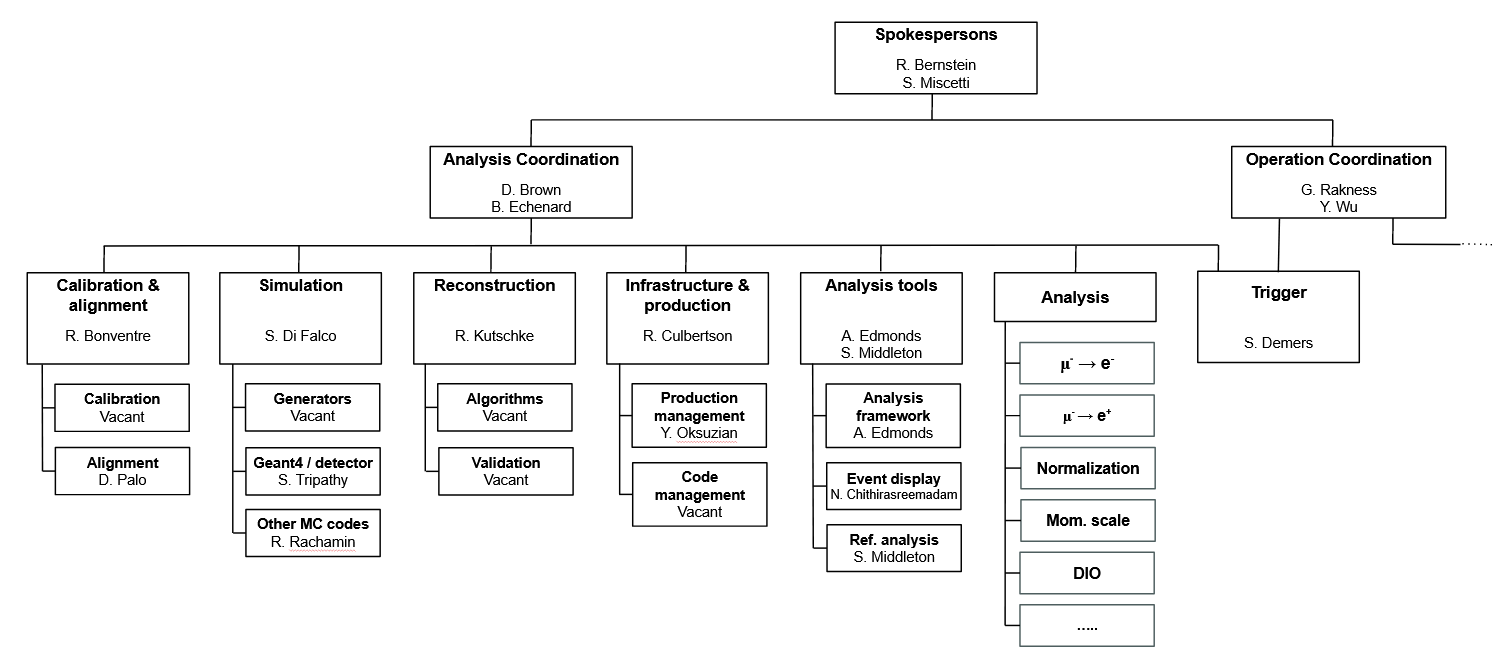
\includegraphics[width=0.9\linewidth]{figures/ACOrgChart.png}
\caption{The organization of the Analysis division within the Mu2e experiment (the sub-structure of operation coordination is not shown for clarity). }
\label{fig:orgchart}
\end{center}
\end{figure}

The Mu2e organization chart is shown in figure \ref{fig:orgchart}. Under the Analysis branch, Offline computing is divided among several Core Groups responsible for providing tools and expertise for the collaboration, ensuring experiment-wide coherence and minimizing duplication of effort. The current staffing of the Core Groups is preliminary, awaiting the introduction of deputies as collaborators complete their Project responsibilities. The five core groups are: 

\begin{itemize}

\item calibration \& alignment. This group supervises the development of Offline tools and procedures to align and calibrate the various Mu2e detector systems and coordinate the data processing required to derive calibration and alignment values. It is also responsible for estimating the statistical and systematic uncertainties on the alignment and calibration parameters, integrating constraints on the overall momentum scale coming from dedicated measurements, and defining the calibration and alignment parameters used in simulation, and the quantities required to monitor the detector response and validate the agreement with the data.

\item reconstruction. This group develops and characterizes the high-level algorithms used to create physics objects (e.,g. background hit removal, track reconstruction, or calorimeter clustering) used in calibration, analysis, and trigger selections. It also ensures that the reconstruction algorithms used in the trigger meet DAQ requirements, and it defines the reconstruction outputs to be monitored in the validation and CI systems. 

\item simulation. The simulation group develops and validates the Monte Carlo generators used to model signal and background components relevant to Mu2e analyses, based on the best available theoretical models and experimental data. This group is also responsible for maintaining the description of the detector geometry and materials in the simulation, and developing Mu2e detector simulations in different Monte Carlo frameworks (e.g. FLUKA) to establish systematic uncertainties inherent to the Geant4 simulation.

\item infrastructure and production. This group manages the offline computing infrastructure and hardware resources to ensure event data, simulated event data, and conditions data are delivered for analysis in a timely and accessible way. It maintains tools to perform data transfer between the online DAQ storage and offline storage, build and distribute the Mu2e software, access data sets catalogs, access and export Mu2e data offsite, maintain offline conditions databases, and perform offline data quality monitoring and continuous integration testing of the Mu2e Offline codebase. It is also responsible for collaborating with CSAID and other resource providers to ensure access to the computational resources and technical expertise required by Mu2e.

\item analysis tools. This group develops the tools required to perform the various physics analyses within the collaboration, including the definition of an analysis framework for the experiment with reduced data formats (aka ntuples), Offline event display(s), and reference analyses to evaluate the impact of reconstruction code developments on the experimental sensitivity and to validate the analysis framework.

\end{itemize}

Additional responsibilities are shared by all groups, such as documenting tools and procedures, developing data quality metrics, or ensuring that the codes meet Mu2e coding standards and performance requirements. A complete description of the core group charges is available in doc-db 48639.





\section{Mu2e Commissioning and Data Taking Plan}
\label{sec:runplan}
Data taking phase descriptions and goals
\subsection{Un-integrated test stand running and Offline computing needs}
\subsection{Cosmic ray commissioning run}

\subsection{Early Beam Configuration}
Low intensity, unstable conditions.



\subsection{ Normal Stable Running Configuration}

The main goal of Mu2e is to detect conversion electrons from muons that stop in the stopping target.  The overall design of the physical apparatus is optimized for this goal.  The normal run configuration will optimize the ability of the experiment to produce and record potential conversion electron events, assuming stable and optimized beams.  A rough description of that configuration is:
\begin{itemize}
  \item Proton beam provided as extracted pulses with good extinction between pulses and reasonable intensity uniformity between pulses (SDF < X)
  \item Proton beam extracted at nominal intensity, focused as tightly as possible on the production target
  \item Detector solenoids at nominal field strength
  \item TS3 collimator set to select a mu- beam
  \item DAQ system configured for data taking in the window 450 -> 1705 ns relative to the nominal proton bunch arrival time at the production target
  \item Onspill Trigger configured for optimal efficiency for recording high momentum (p>80 MeV/c) electrons and positrons.
  \item Remaining Onspill trigger and data handling bandwidth allocated to dedicated calibration channels
  \item Offspill trigger configured to record cosmic rays useful for background estimation and detector calibration and alignment
\end{itemize}

\subsection{Special Runs}
There are several special running configurations that Mu2e will use to enhance non-conversion electron signals that are inaccessible or greatly attenuated during normal stable running configuration, but which are valuable for estimating physics backgrounds to conversion electrons.  Special run configurations will also be necessary when them beam conditions are non-optimal.  Some non-beam calibration run configurations will also be used.  These are described below.

unstable beam minimal feedback configuration.

RMC and RPC configuration
pi e nu configuration
mu Michel edge configuration

\subsection{Calibration Run Configurations}
calo source calibration config.

\subsection{Run 1}
Goals and parameters of run 1.
\subsection{Run 2}
Goals and parameters of run 2.

\section{Offline Computing Model Overview}
\label{sec:overview}

%The Mu2e Offline Computing Model describes the software, infrastructure, tools, and workflows to store, process, simulate, and analyze data. Offline covers all computing activities except data acquisition; Online computing and the data acquisition system are not included in this scope, but a summary is provided in section~\ref{sec:daq} to introduce the concepts and terminology used in the rest of this document. The formal interface between Online and Offline lies at the DAQ buffer disks in the Mu2e building. Online is responsible for writing data on these disks, and Offline is in charge of transferring the files for further processing (and safely deleting them on the buffer disk). 

%The Offline Computing Model is based on the framework and tools provided by the FNAL scientific computing division (SCD), the Fabric for Intensity Frontier Experiments (FIFE) group, and global infrastructures such as the Open Science Grid (OSG) or High-Performance Computing (HPC) centers. The event processing framework is built on the {\it art} framework developed by SCD, supplemented by Mu2e-specific algorithms, a condition system, a geometry description, and the definitions of data products. All calibration, reconstruction, and simulation algorithms operate within this environment. This code base is usually referred to as Mu2e Offline (or just Offline). This model has been in development for more than a decade, from characterizing the detector performance in the TDR and CD-3 phases to the most recent estimate of the experiment sensitivity~\cite{Mu2e:2022ggl}. At each stage, the model has evolved to manage the growing processing requirements and the increasing complexity of the simulation and reconstruction tasks. This model will continue to mature to take advantage of future computing technologies and infrastructures as well as advances in computational techniques over the coming decade. 

The Mu2e Offline Computing Model (OCM) describes the software, infrastructure, tools, and workflows to store, process, simulate, and analyze data. This definition covers all computing activities downstream of the data acquisition process. The DAQ system and Online software are not included in this scope, but a summary is provided in section~\ref{sec:daq} to introduce the concepts and terminology used in the rest of this document. The formal interface between Online and Offline lies at the DAQ buffer disks in the Mu2e building. Online is responsible for writing data on these disks, and Offline is in charge of transferring the files for further processing and safely deleting them on the buffer disk. 

%Mu2e is a medium-scale collaboration with moderate computing needs compared to large-scale experiments, but also a lower level of resources. 

The OCM is devised to support Mu2e physics goals by designing systems minimizing operations effort, addressing anticipated obstacles, and aligning with the host laboratory tools, support, and strategy. This system is based on the framework and tools provided by the FNAL Computing Science and Artificial Intelligence Division (CSAID) and the Fabric for Intensity Frontier Experiments (FIFE) group for small- and mid-scale intensity frontier experiments. The computing resources are mostly provided by the host laboratory in the form of conventional UNIX batch systems accessible via the Open Science Grid (OSG), supplemented by external resources whenever available (e.g. high-performance computing centers). However, several hurdles limit the use of external resources. They are usually not controlled by Mu2e, or even HEP, and might be subject to annual applications and restrictions. Some centers may also have limited network connectivity, making it difficult to move large amounts of data in a reliable manner. In these instances, performing computing tasks with large CPU/IO ratios (e.g. simulation) may be more advantageous. Finally, High Performance Computing Centers (HPCs) are very diverse in the hardware offered and might require significant software development effort to use specific resources efficiently. The overall Mu2e computing strategy is, therefore, to store all raw, reconstructed, and simulated data at the host laboratory to perform most of the simulation, reconstruction, and calibration tasks. External resources are exploited whenever available to perform non-critical tasks, such as simulation or data reprocessing, privileging CPU-intensive operations. Reduced data sets of modest size are also produced to enable data analysis at local institutions. 

One of the main components of the OCM, the event processing framework, is built on the {\it art} framework developed by SCD, supplemented by Mu2e-specific algorithms, a condition system, a geometry description, and the definitions of data products. This code base is usually referred to as Mu2e Offline (or just Offline). This model has been in development for more than a decade, from characterizing the detector performance in the TDR and CD-3 phases to the most recent estimate of the experiment sensitivity~\cite{Mu2e:2022ggl}. At each stage, the model has evolved to manage the growing processing requirements and the increasing complexity of the simulation and reconstruction tasks. This model will continue to mature to take advantage of future computing technologies and infrastructures as well as advances in computational techniques over the coming decade. 

The workflow designed for the OCM starts with the data written by the DAQ system on the buffer disk. At the beginning of each run, the DAQ system copies all information used to configure the detector and DAQ into the online run conditions database. The online content is periodically streamed to an offline database instance. As new runs appear in the online database, the raw data are transferred from the DAQ storage disk to a disk visible to Offline worker nodes. There are about 15 independent data streams but these may be packaged into fewer files due to constraints from the TDAQ system and data movement capabilities. A first pass (\passone) of Offline reconstruction is triggered with minimal latency. This \passone\ uses the reconstruction results to produce updated calibration constants and offline data quality metrics, persisted in the corresponding databases. The data are then reprocessed (\passtwo) with the updated calibration conditions. Reconstructed data objects from both passes are stored to tape and registered in a file catalog. A blinding scheme will be developed and applied to data released to collaborators to avoid any implicit experimental bias. In specific cases, e.g. if substantial improvements to either the reconstruction codes or calibration values, a complete data reprocessing of all data will be done. Finally, reduced data sets (aka skims and ntuples) are produced for further analysis. This workflow assumes 8/5 support for offline databases, with best effort outside standard hours.

Mu2e events are selected by trigger algorithms based mostly on information from the tracker and calorimeter. The low-level digital data coming from each subsystem are first converted into physical objects using calibration data (e.g. objects providing a physical time, position, energy, etc.). A set of algorithms then filters and aggregates these hits into increasingly complete physical objects. A two-step clustering algorithm is used to form calorimeter clusters from crystal hits, including a procedure to recover split-off clusters. The track-finding algorithm starts by filtering hits produced by low-energy electrons with dedicated algorithms, then identifies clusters of hits with a short time window (typically $\sim$50 ns). These hits are passed to helix finding algorithms to extract an approximate helix parameterization. One algorithm uses the position of high-energy calorimeter clusters and the stopping target to seed the helix search, while the second is purely based on tracker information. The calorimeter-seeded algorithm tends to be more robust against higher levels of background but has inherently lower efficiency. Reconstructed helices are finally passed to a Kalman filter track fitter. Two configurations have been developed for the Mu2e KinKal fit, one optimized for use in the online trigger, and a second for offline analysis. Physics and calibration data are selected by a set of trigger filters based on the reconstructed tracks and calorimeter clusters, with adjustable prescale factors to tune the total trigger rate. Data from the extinction monitor and stopping target monitor are reconstructed in dedicated applications. Their final outputs are associated with the corresponding event data by their DAQ timestamp. 

Complete end-to-end simulations of Mu2e datasets are prohibitively expensive to produce directly given the huge number of protons on target. Current samples were produced by splitting the processing into pileup, signals, and physics backgrounds. Geant4 is used to model the Mu2e experiment and particle interactions. Pileup is simulated starting from protons hitting the production target, recording the proton daughter particles as they exit the Transport Solenoid. Daughter particles are re-simulated (resampled) many times to increase the effective statistics, limited by the eventual repetition of the same daughter particles (oversampling). Current pileup samples were produced with a $\sim 10$M core hour campaign, producing roughly 1 second of pileup at the expected nominal Mu2e intensity. Muon-based signals and physics backgrounds are simulated starting from stopped muons recorded during the pileup simulation, which are resampled many times, forcing them to decay via a desired physics process. Stopped muons are plentiful in the pileup sample, and existing muon-based signal and physics background samples are many times larger than what Mu2e might observe in the region of interest. Cosmic ray backgrounds are simulated starting with standard generators (CRY, CORSIKA), stopping and resampling the particles entering the CRV. Current samples correspond to roughly 3 times the expected \runone sky live-time. The net output of the pileup, signal, and physics background simulations are energy deposits in the Mu2e detector. Simulated samples of raw on-spill data are created by mixing samples of pile-up and signal/physics background scaled to the expected beam intensity average and fluctuations. The different sources are finally mixed to produce a realistic sample, and processed with the same reconstruction code used to produce the data. 

Tools and policies are in place for code management, code review, building code, code validation, release management, release distribution, setup of the development environment, and setup of the runtime environment. For example, the code base is maintained in Git repositories, and the GitHub pull request system is used to control and review contributions to the code base. The SCD-supplied CMSBOT software is also used for the launch tests that are executed on the SCD Jenkins system. These tools will continue to evolve to integrate changes in the supported product stack by SCD and FIFE. Calibration data are stored in condition databases, indexed by (fraction of) runs, and grouped into intervals of validity. The metadata needed to access and process data (DQM, MetaCat, Rucio, luminosity,...) are stored in several dedicated databases. All databases are supported by the database group of the FNAL IT division. 

The analysis model is designed to be lightweight and flexible. Information about Mu2e events will be provided to users in the the form of ROOT ntuples containing a simplified output of the full reconstruction algorithms (while we expect the vast majority of analysts will use reduced data sets, analyses could still be conducted within the full framework). These reduced datasets require much less storage, facilitating data analysis on local resources and reducing the development time of analysis pipelines. A Python interface and a common analysis environment will also be provided to facilitate the inclusion of external tools (e.g. machine learning or statistical tools). In addition, several event displays are available to visually inspect individual events and help design analysis codes.

To this day, generators for all of the relevant signal and background processes exist and have been exercised in Mock Data campaigns. Reconstruction algorithms exist for all of the Mu2e detectors, with the majority of detector response functions tuned to measured data. Most of these algorithms are highly advanced and in nearly final form, where further optimization requires actual data. Many detector calibration algorithms have been demonstrated using bench test data and simulations. In many cases, these are fully developed, while in others they constitute only proof of principle. Some algorithms still require further development to meet the performance requirements. However, none of the missing calibrations are critical to triggering, recording, or evaluating the quality of Mu2e data, but will be required for precision physics analyses. 

Procedures to automatically process raw data as they appear from the online system exist and have been demonstrated to meet requirements, using data from bench tests and simulations. A conditions database and file catalog system based on the central tools currently supported by CSAID are in active, daily use, and have been exercised at scale in simulation campaigns. Operation of Geant4 in multithreaded mode on HPC resources has been demonstrated. The performance of the Offline processing has been benchmarked using preliminary estimates of the data volumes the Online system will produce, and shown to fit within the processing and storage envelope agreed with FNAL central computing. Configurations of the Offline algorithms run as part of the Online software-based event selection process (trigger) are in an advanced development stage and have been shown to meet requirements for \runone operations.

Code development adheres to industry standards and best practices, following a continuous integration (CI) model in which changes are frequently integrated into the source code. All changes are done via pull requests reviewed by experts and validated with a series of quality checks before integration. Database development is fully integrated with this workflow and synchronized with software releases. Prototype analysis interfaces to the Mu2e data have been developed and are in active daily use for developing analyses and calibration algorithms.
\section{Event Data Handling}
Describe the event data handling model from when it appears Offline (from DAQ) to analysis.  This should be largely stolen from the RDM document 39531.

\section{Simulations}
\label{sec:simulation}

Prior to the start of operations, the main purpose of Mu2e simulation was to verify the expected performance of the experiment and to allow optimization of the detector design. That required an accurate, detailed, and flexible model of the experiment. In the analysis phase, the simulation will be used to optimize alignment, calibration, and reconstruction algorithms, to estimate the expected detector acceptance and resolution, and to develop analysis algorithms. The Mu2e simulation was designed to satisfy both of these objectives.

The Mu2e simulation is based on the Geant4 framework~\cite{geant4:2003,geant4:2006,geant4:2016}, including a description of the {\em as built} geometry and the material composition for both the sub-system parts and the experimental hall; the temporal and spatial structure of the proton beam; magnetic field maps; the implementation of the detector response as measured at beam tests and with cosmic rays; and a complete interface with the calibration database. A set of custom event generators dedicated to the conversion electron channel and the main sources of background are also used, and full events are simulated with overlapping beam background particles. Additional studies have been performed using other Monte Carlo codes (MARS\cite{MARS:2009}, MCNP\cite{MARS:2009, MCNP:2012}, FLUKA\cite{FLUKA:2013}, PHITS\cite{PHITS:2018}) to validate Geant4 predictions and to estimate their uncertainty.

The following sections describe the simulation workflow, the detector modeling, the physics generators, and the production campaigns in more detail.


\subsection{Simulation workflow}
The simulation of the large number of events expected in Mu2e requires some optimization of the processing time. This is achieved with a staged simulation approach together with resampling techniques. Given the statistical nature of the particle interactions in the material crossed before reaching the detectors, it's possible, where appropriate, to reuse many times the particles stored at the end of one stage ({\em resampling}) increasing the available statistics at a reduced cost of CPU time. The absence of statistical biases ({\em oversampling}) must be checked case by case. The staged approach helps to save additional CPU time when no changes occur in the first stages and it's sufficient to rerun only the last stages. In addition, different particle range cuts can be used in each stage to avoid unnecessary particle tracing. 

The main beam simulation is divided into four stages:
\begin{enumerate}
\item from the 8 GeV proton beam on the Production Target (PT) to the entrance of the Detector Solenoid (DS);
\item from DS entrance to the stopping target;
\item from the stopping target to the exit from the DS volume (tracker, calorimeter, and cosmic ray veto hits are stored);
\item detector response and digitization.
\end{enumerate}

The initial beam protons are given the nominal beam energy and direction, distributed across the PS entrance as a symmetric Gaussian with the width expected from beam simulations. The time of each proton is sampled from a distribution generated by detailed simulations of the slow extraction and active extinction system. To save processing time, charged particles that exit the PS volume forward are killed.

Special workflows have been developed to optimize the production of dedicated samples as well. Pion decay can be disabled to increase the number of stopped pions in the stopping target, and the stopped pion probability is then corrected for the pion survival probability depending on its lifetime. The first stage of the antiproton simulation has also been divided into four phases to use a customized differential cross section for antiproton production and optimize the absorber window located at the center of TS. The cosmic ray simulation requires a dedicated workflow as well. In the first stage secondaries produced by the CRY generator~\cite{CRY:2007} according to the flux at sea level are traced from the top of the Mu2e building to the DS. Events are divided into three categories according to the energy deposited in the Cosmic Ray Veto (CRV): high (E>16 MeV), low (E<16 MeV), or null (neutrons or particles passing through the TS hole). In the following stage, particles are resampled and traced through the detector. Finally, digitization is performed. In all cases, only the events with a minimum energy deposit in the tracker, the calorimeter, or the cosmic ray veto are passed to the digitization stage.


\subsection{Event generators}
A set of generators has been realized to have a more accurate simulation of the particle yield from the stopping target. Starting from the position and time of the stopped muons or pions, the following single particles can be generated with isotropic direction: conversion electron (Leading Log spectrum~\cite{Czarnecki:2011mx, Szafron:2017guu}), conversion positron (Leading Log spectrum~\cite{Czarnecki:2011mx, Szafron:2017guu} rescaled to the expected peak momentum of 92.3 MeV/c), DIO (Leading Log spectrum~\cite{Szafron:2016}), muon capture secondaries (protons and deuterons spectrum adapted from Ref.~\cite{TWIST:2020, ALCAP:2022}, neutron spectrum adapted from Ca measurements~\cite{MCnspectrum:1978} and normalized according to Ref.~\cite{MCnnorm:1965}, x-rays and gamma rays used to study the Stopping Monitor response are generated as single lines), radiative muon capture secondaries (photon spectrum from the fit of experimental data~\cite{TRIUMF:1999} with the closure approximation~\cite{closureapprox}), radiative pion capture secondaries (photon spectrum adapted from Mg data ~\cite{Bistirlich:1972}). Cosmic ray studies are performed with the CRY generator to evaluate the cosmic background and the CORSIKA generator~\cite{CORSIKA:1998} to estimate the uncertainty on flux normalization. A custom generator to produce antiprotons from protons interaction in the production target has been developed fitting the existing data and extrapolating them to the 8 GeV Mu2e beam energy~\cite{Mu2e:2022ggl}.

\subsection{Pileup simulation}
In addition to simulating particles of interest for physics studies and calibration, Mu2e must model the pileup of the many low energy particles produced by beam particles and decay/capture products of the vast majority of stopped muons which do not convert to electrons, or produce a particle which could be a signal background. Pileup is not itself a source of background for physics analyses, but the detector signals it generates can significantly affect the reconstruction efficiency and/or resolution of signal-like particles.

Mu2e simulates pileup using Geant-4, starting with protons hitting the production target (POT), as described above. Charged particles traveling backward and entering the TS are check-pointed as they enter the DS. Neutral particles that exit the beamline are check-pointed as they exit the TS or PS volume.

In subsequent simulation jobs, each check-pointed particle's passage through the DS is resampled 1000 to 10000 times, depending on the sample. Particles producing energy deposits in the detector sensitive volumes are saved, along with their genealogy and energy deposits. To allow correct normalization when used downstream, the fraction of saved events is calculated automatically during the resampling, relative to the original number of simulated POT, and stored in the conditions database.

Resampled muons stopping in the stopping target are check-pointed before they decay and then resampled 10000 times in turn to model pileup from muon capture and decay daughters. The muon lifetime is randomly sampled for each resampling, and custom codes are used to randomly select a decay mode. These same check-pointed target-stopped muons are also used as starting space points in the signal generators described above. The efficiency of resampled stopped muons producing energy deposits in sensitive volumes is computed and recorded in the database. 
The breakdown of signals expected from simulated pileup by time and stream in individual Mu2e detector sensor elements (straws for tracker, etc.) is shown in Fig.~\ref{fig:sim_pileup}.

\begin{figure}[ht!]
\centering
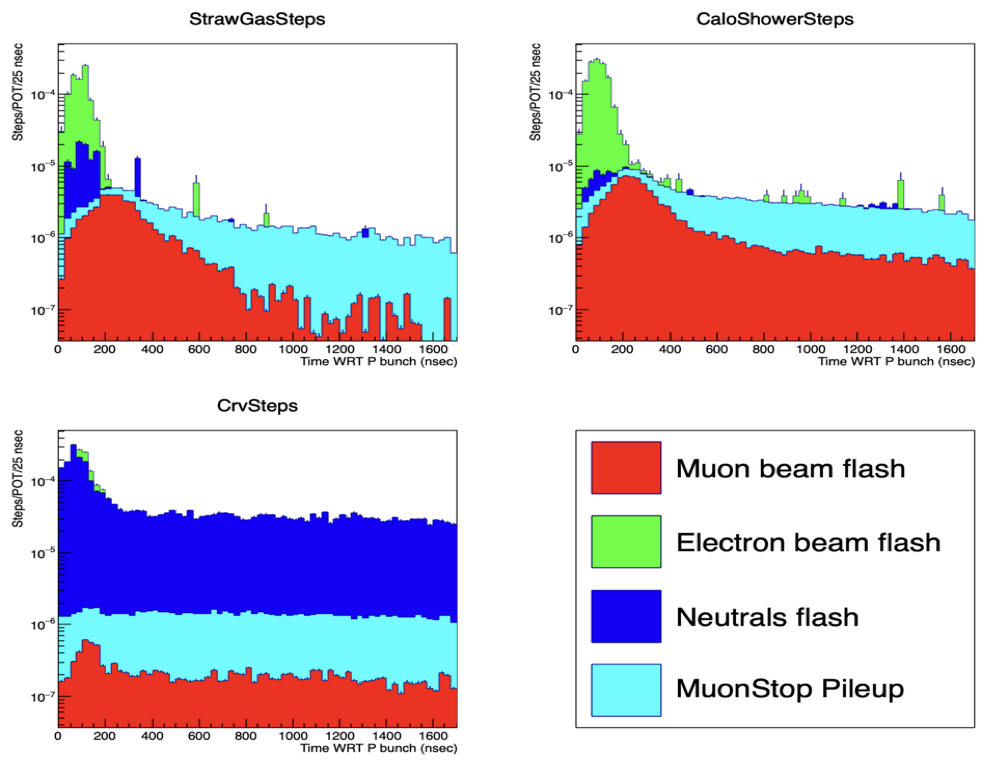
\includegraphics[width=0.8\textwidth]{figures/sim_pileup.png}%
\caption{Simulated signal counts in individual detector elements (steps) per POT relative to the arrival time of protons on the production target, wrapped to the beam pulse period, for the four pileup streams described in the text.}
\label{fig:sim_pileup}
\end{figure}

Pileup in the CRV is dominated by the neutral particles (mostly neutrons) leaving the PS. As the cross-section for generating signals in the CRV is small, these can be resampled many times, currently 10000. A physics list including detailed neutron interactions is used for this stage. Neutral CRV pileup resampling dominates the resources needed for pileup simulation, as the required statistics are large and the processes involved are time-consuming to model.

Pileup is overlaid on signal events by adding the sensitive volume energy deposits from an appropriate number of pileup daughters to the energy deposits generated by the signal process particle. Pileup data are read through art secondary input streams, in sequential mode, starting from a random starting event.
The number of pileup daughters needed is computed for each event by sampling the expected POT distribution, scaling that by the products of the relevant resampling efficiencies read from the database, and then applying Poisson fluctuations. The resulting summed energy deposits are then passed through the detector response simulation. Since the proton pulse intensity is expected to be relatively constant over millisecond timescales, and the pulse trains are long, the time of each pileup particle energy deposit is wrapped around the 1695 ns bunch period when summing.

Most Mu2e pileup simulations use a POT intensity distribution modeled by a log-normal distribution with Spill Duty Factor (SDF) = 60\%~\cite{Mu2e:2022ggl}, scaled to the average beam intensity expected for operations with either 1 or 2 booster batches. A time sequence of POT computed using a detailed beam extraction simulation can also be used.
The workflow for pileup simulation from POT and subsequent mixing onto simulated signals is shown in Fig.~\ref{fig:dts_mixing}.

Even when leveraged by resampling, simulating pileup from POT is very inefficient. Using $\sim7M$  core-hours of processing time, the most recent simulation campaign produced roughly 5 seconds (1.3 seconds) of experiment running time (beam live time). These samples also show statistical artifacts due to over-sampling of some particles. To avoid these limitations, Mu2e is developing code to overlay pileup extracted from beam data on simulated signals. By triggering randomly, Mu2e can record essentially unlimited pileup events with essentially zero resource cost that will naturally track the real POT intensity, and follow changing detector conditions. Unlike simulated signals and pileup, which are merged prior to digitization, pileup from beam data will be already digitized. Digital pileup that don't overlap with simulated signal particle energy deposits in time or channel can be merged trivially. Digital pileup that overlaps in both time and channel with simulated signals will be handled by dedicated codes. For the tracker, at the expected nominal beam intensity with 1 booster batch, 98\% of pileup signals are non-overlapping. 

The event identity of mixed (digital) pileup plus simulated (signal) events is given by the simulated event, to allow digitized pileup frames to be reused, and to distinguish them as Monte Carlo. Most conditions data used in simulating the signal and reconstructing the combined event are keyed to the pileup. This includes dead or noisy channels, sensor and electronics response, and resolutions. For effects which are not simulated, such as individual straw miss-alignments, conditions data are taken from the simulation. Preliminary studies overlaying digitized simulated pileup on simulated conversion electrons, using a very naive overlap resolution algorithm, shows nearly identical results post reconstruction as energy deposit pileup overlay. Digital pileup overlay is currently only implemented for the tracker. Extension of the digital pileup overlay algorithms to include the calorimeter and CRV, and development of more sophisticated algorithms for treating overlapping signals, as planned for the immediate future. The workflow for mixing pileup from random triggers onto simulated signals is shown in Fig.~\ref{fig:dig_mixing}.

\begin{figure}[ht!]
\centering
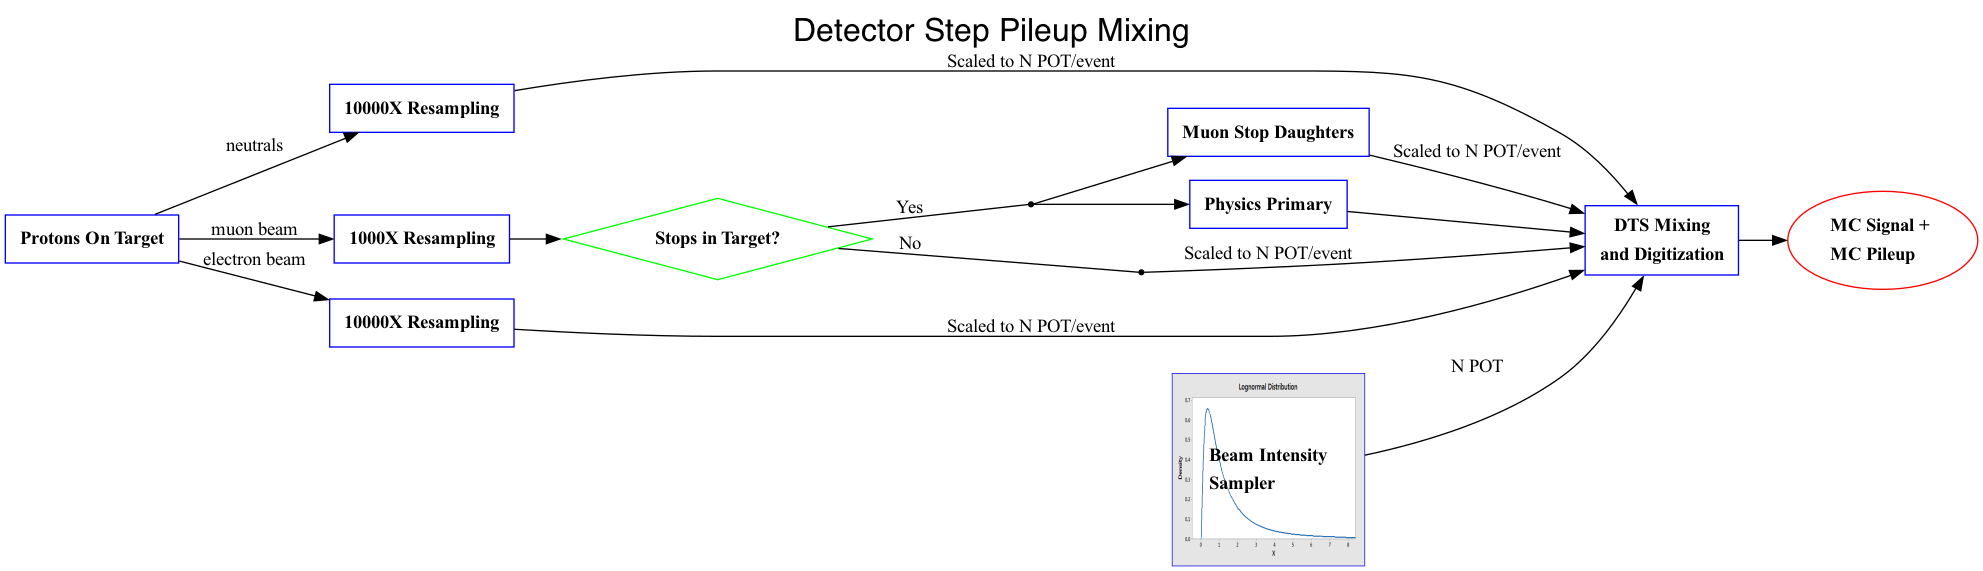
\includegraphics[width=\textwidth]{figures/DTS_Mixing.png}%
\caption{Workflow for producing simulated signal events with overlaid simulated beam pileup.}
\label{fig:dts_mixing}
\end{figure}

\begin{figure}[ht!]
\centering
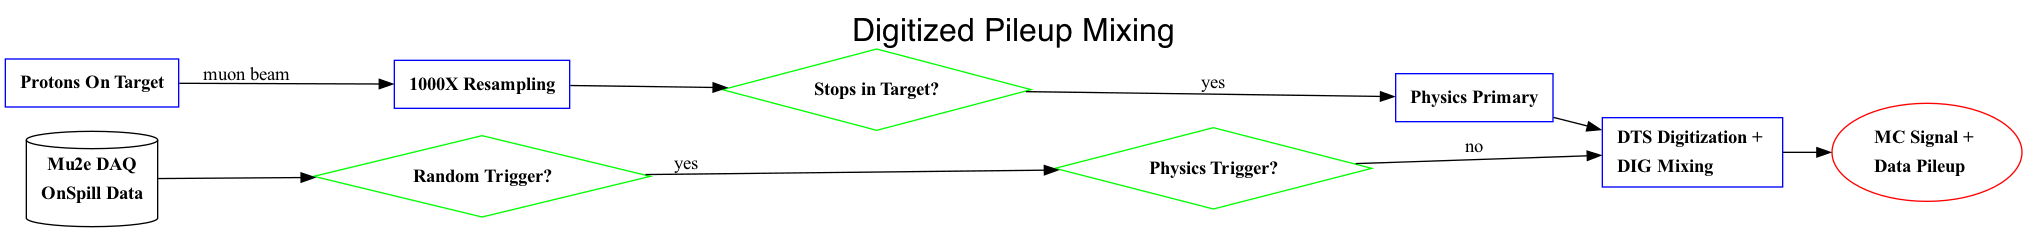
\includegraphics[width=\textwidth]{figures/DIG_Mixing.png}%
\caption{Workflow for producing simulated signal events with overlaid beam pileup extracted from data.}
\label{fig:dig_mixing}
\end{figure}

\subsection{Geant4 Physics processes}
The main physics interactions are simulated using a modification of the GEANT4 "Shielding" physics list. The main modification consists of increasing the threshold used to pass from the Bertini Cascade (BERT) model for low energy hadron-nucleus interactions to the Fritiof (FTF) model from 4-5 GeV to 9.5-9.9 GeV to better reproduce the experimental data on pion production. Nuclear de-excitations and radioactive decay of long-lived isotopes are included. Hyperon and anti-baryon production is obtained from the chiral invariant phase space model (CHIPS). Neutron simulation uses the high precision model (HP) up to 20 MeV. This is particularly relevant for the prediction of the thermal neutron background.

Geant4 is used only to produce the electrons and the photons from the atomic cascade to the ground state for muon capture in the aluminum stopping target. The nuclear muon capture, the muon decay in orbit, the radiative muon capture, and the muon conversion are simulated using custom generators (see below). The same holds for the radiative pion capture in the stopping target. Simulation of muon and pion captures outside of the stopping target is generally managed by Geant4, but custom generators have been created for particular studies related to detector calibration.  

Additional Monte Carlo codes are used to validate and evaluate systematic uncertainties in the predictions of critical quantities obtained with Geant4. MARS has been extensively used to study the radiation levels in the Mu2e hall, the effectiveness of the concrete shielding and of the Heat and Radiation Shield, and the dose and neutron fluence in the tracker and calorimeter electronics. The effect of concrete shielding on neutron and kaon radiation has also been studied with FLUKA and MCNP. Pion production in the PT has been investigated with MARS, MCNP, FLUKA, and PHITS, while Geant4 expectation for antiproton production in the production target has been corrected given its disagreement with MARS, MCNP, and FLUKA~\cite{Mu2e:2022ggl}. 

\subsection{Geometry description}
The experimental hall as designed for the first run of the experiment is shown in Fig.~\ref{fig:mu2e_geom}. The main information obtained from the simulation of the passive parts is the effectiveness of the shielding against the radiation produced by beam interactions and cosmic rays. The simulation includes the dirt surrounding the detector hall, the building walls, the concrete shielding blocks, the solenoids warm and cold mass, the radiation shield, the mechanical structure of the tracker and calorimeter, the beam dump downstream of the proton beam with the extinction monitor, ... The amount, type, and location of shielding have been decided as a compromise between budget considerations and the amount of radiation acceptable for the different sub-systems. It will be reviewed for Run II according to the result of Run I.
 
The geometrical description of each sub-system is maintained by the corresponding working groups. The level of detail of the geometry description is a compromise between the time needed to simulate the events and the agreement between data and Monte Carlo simulation. The main parameters (e.g. material composition, number of elements, single element dimension, and location) are included in the geometry database. The dimensions and positions of the active parts (tracker straw tubes, Ecal crystals, ...) are the nominal ones: mechanical tolerances, gravitational sags, or misalignments are introduced at the digitization level.

A separate geometry package has been realized for the detector commissioning with cosmic rays. The simulation of the experimental setup in this {\em extracted position} includes the tracker and calorimeter out of the Detector Solenoid and a few modules of the Cosmic Ray Veto on top of them (Figure~\ref{fig:mu2e_geom}(right)). Alternative geometrical descriptions for the detector have been realized using MARS and FLUKA to determine the uncertainty of simulation estimates of the radiation levels and the stopped muon yield.

\begin{figure}[ht!]
\begin{center}
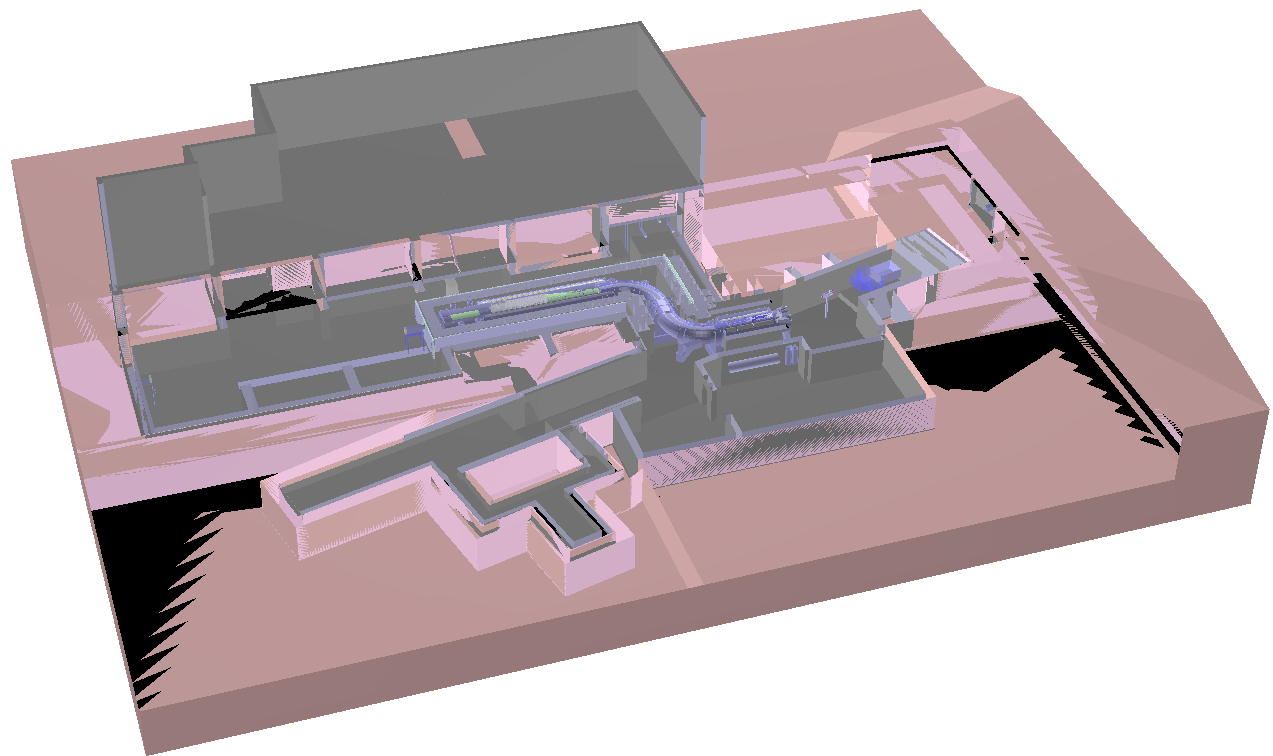
\includegraphics[height=0.29\linewidth]{figures/mu2eHall.png}
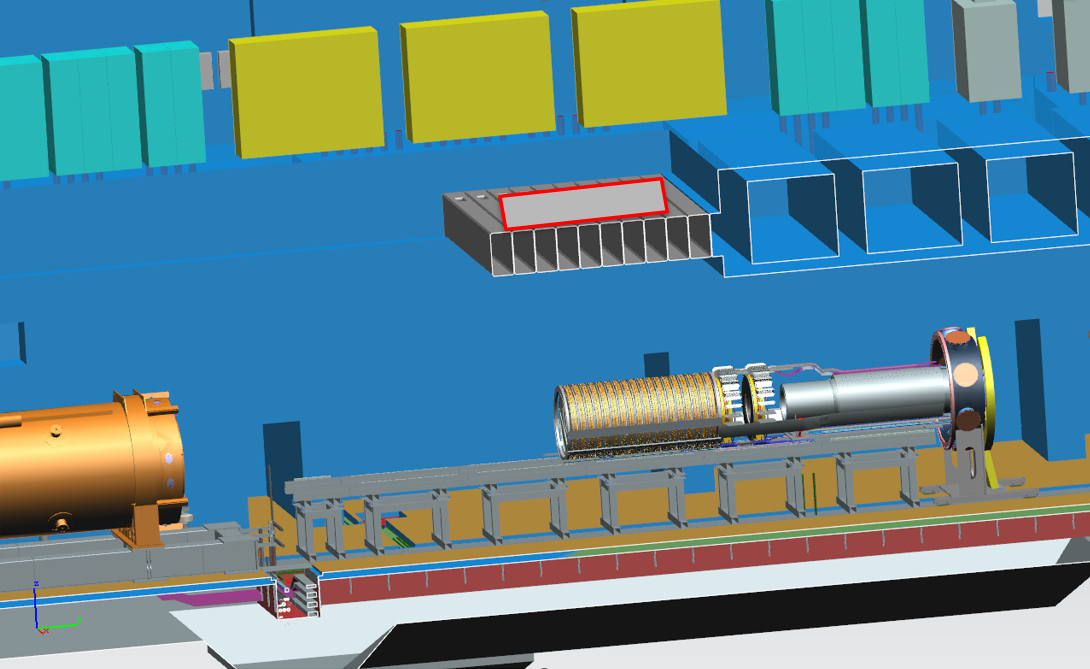
\includegraphics[height=0.29\linewidth]{figures/geom_extracted.png}
\caption{Left: the Mu2e experiment and building in the Geant4 Offline simulation. Right: Mu2e detectors in the extracted position.}
\label{fig:mu2e_geom}
\end{center}
\end{figure}

%Each sub-system group has developed the geometry description of the setup used for beam or cosmic ray tests of the prototypes or for the Vertical Slice Test of the first production modules. Although these are in general standalone programs, they have been an important tool to validate the detector description in the Offline repository. 

\subsection{Magnetic field maps}
Detailed magnetic field maps are produced using the OPERA 3D~\cite{opera3D} and HELICALC~\cite{helicalc} software packages using (warm) as-measured conductor geometries and coil positions provided by the Mu2e project solenoid construction team. The field is stored as a discrete vector map over a Cartesian grid, separately for the Production Solenoid (PS), Transport Solenoid (TS), Detector Solenoid (DS), and the region outside all the solenoids. The effect of re-bar in the concrete shielding has been calculated but not yet included. Field maps for special run conditions used for calibration purposes have also been generated. The field map is accessed through a software interface that dynamically interpolates the field vectors from the 9 grid points nearest the requested reference point.

The Mu2e operations team will determine the in-situ DS magnetic field using a custom survey device that will measure the magnetic field components at fixed locations within a cylindrical coordinate grid. A fit to the measured data using a combination of a multi-pole expansion and relaxation ANN constrained to Maxwell's equations will be used to interpolate and average the measurements into the Cartesian grid format. This map will be corrected for the estimated effect of re-bar in shielding materials that can't be in place during the field survey.

Publication quality simulations and reconstruction will use the field map determined from the survey. Changes in physics objects reconstructed using alternative maps spanning the measurement and shielding magnetization uncertainties will be used to estimate the systematic errors on physics measurements due to residual field map uncertainties.


\subsection{Detector response}
Each sub-system has a dedicated simulation of its digitization. This includes a parameterization of the physics processes bringing the signal from the position where the energy is deposited to the readout electronics and also the simulation of the electronics response. Simulated digitization uses the timing information from the (simulated) DAQ clock system used to define the start and stop of each digitization period, including the 5-fold repeating pattern of different event start times and lengths caused by the period mis-match of the booster and the delivery ring clocks.
%\red {So we foresee to use some database information during digitization?}

\begin{itemize}
\item{Tracker -} energy deposits in the straw tubes from different particles are collated and processed by applying a parameterized simulation of the drift time, gas amplification, signal transit time along the wire, electronic amplification, and shaping. Electronic signals at the straw ends are superimposed and the resultant waveform is digitized. Only digitized hits passing the discrimination threshold at both ends are saved. 

\item{Calorimeter -} energy deposits in each crystal are grouped in time. The number of photons produced by scintillation takes into account the average light response uniformity measured during crystal qualification. The number of photo-electrons obtained using the average PDE of the SiPMs is smeared with a Poisson distribution. The digitizer waveforms corresponding to energy deposits in the same readout unit are superimposed. Radiation-induced noise and electronic noise are added. Zero suppression is reproduced.

\item{Cosmic Ray Veto -} energy deposits in each module are grouped in time. The bunch time structure is applied (only for the on-spill simulation). The time distribution of the charge collected by the SiPMs located at the edge of each module is calculated using the scintillator light yield, the WLS collection efficiency, the light attenuation along the fiber, the reflection probability on the walls, and the SiPM photon detection efficiency. The charge collected by the SiPMs is transformed into signal waveforms after applying a random time jitter and photo-electron fluctuation. ADC and TDC counts are obtained by applying waveform sampling and discrimination. 

\item{Stopping Target Monitor -} energy deposited by each photon in the HPGe detector is used to generate a waveform according to the deposited ionizing energy, measured gain, and collection efficiency. Waveforms from different photons are superimposed using the expected time and energy distribution. Electronic noise from the pre-amplifier and amplifier is added. The resulting waveforms are digitized using the 16bit ADC, and are used together to form STMWaveformDigis. A similar technique will be used for LaBr response.

\item{Extinction Monitor -} energy deposits are converted into electron-hole pairs. The number of charge carriers is fluctuated using the silicon Fano factor of 0.1. The deposited charge is split into a number of clusters uniformly distributed along the particle path inside the sensor. Each cluster is drifted individually. The sum of the charge reaching the pre-amplifier with its time structure is passed to a discriminator that simulates the time and time over threshold response of the readout chip. At the final stage, the digitization algorithm adds random hits to the output~\cite{ExtMon:2014}.
\end{itemize}


\subsection{Simulation campaigns}
Several simulation campaigns have been conducted since the inception of the experiment to guide the design and evaluate the corresponding physics performance. The SU2020 campaign was based on workflows developed in 2018, and the output was used to update the sensitivity estimate of the experiment for expected run 1 operations. That work pulled in effort from a number of younger collaborators, and was published \cite{Mu2e:2022ggl}.  The most recent campaign, MDC2020, used updated geometries, detector response simulations, and a streamlined workflow to generate
large samples of beam, pileup, signals, and physics backgrounds. The principal output of MDC2020 was a large sample of conversion signals with pileup, used in algorithm development, plus pure pileup events, for trigger studies.
MDC2020 used the Production Operations Management Service (POMS) to run complex grid campaigns, and GitHub to store scripts and configuration files. The whole effort was driven by the Mu2e Production Manager. 
Different sets of calibration and alignment conditions were simulated to evaluate their impact on the reconstruction efficiency. Most of the conditions were also directly extracted directly from the database, providing a test of the condition system in a production setting. These data have proved essential to improve and evaluate the performance of reconstruction algorithms, including those used in the trigger, and perform the SU2020 sensitivity study~\cite{Mu2e:2022ggl}. 

\subsection{Ensembles}
\label{subsec:ensembles}
While useful for software development and some physics studies, individual background streams produced in MDC2020 are not representative of the mixed-signal samples that will be used for analysis. Mock Data samples were introduced to provide a more accurate model of what Mu2e will record during data-taking phases. These samples are produced by merging individual background sources (Pile-up, cosmic rays, DIO, RPC, ...) into a data collection with mixed content, according to event event fractions expected in real data. The combined sample is then passed through our digitization and reconstruction framework to create "data-like" samples. Ensemble creation uses a dedicated art input module that knows how to sample multiple input files. In addition to the development of calibration procedures and analysis frameworks, the ensemble data sets will also enable test of the computing infrastructure in more realistic conditions. Production of large ensemble data sets for dry-run tests of the offline calibration and processing workflow at scale is foreseen before the start of Mu2e beam running.
\section{Event Reconstruction}
\label{sec:reconstruction}

Algorithms for converting Mu2e raw data into physics objects (i.e. reconstruction) have been in development for over 14 years. Operating on the output of the detailed simulations described in section \ref{sec:simulation}, these algorithms have been used to quantify the expected performance of the detector \cite{TDR} and the physics reach of the experiment \cite{Mu2e:2022ggl}. The output of reconstruction is used to perform the high-level calibration and alignment discussed in section \ref{sec:calibration}, and as the basis of the physics analysis processing described in section \ref{sec:analysis}. 

Reconstruction of the Mu2e primary event data stream proceeds in several stages. First, the low-level digital data (digis) coming from each Mu2e subsystem are converted into hit objects, which present the equivalent information in physical units, using calibration objects from the conditions service (see section~\ref{sec:databases}). A sequence of algorithms then aggregates and filters these hits into increasingly complete and accurate representations of physical particle candidates. The final versions of these particle candidates, with their ancillary information, are stored for downstream analysis. The reconstruction sequence relies on AI/ML at several stages, pointed out in the text.

Data from the extinction monitor and stopping target monitor are reconstructed in dedicated applications. Their final outputs will be recorded in the conditions database, associated with the corresponding event data by their intervals of validity. Reconstruction algorithms are currently under development.

All Mu2e reconstruction is implemented within the art framework~\cite{Green:2012gv}. Raw data from the DAQ system are stored as compressed digitizations with associated headers, called fragments, which are reformatted into Offline digi collections before reconstruction begins. Simulated data are produced directly as Offline digi collections. Individual reconstruction stages are implemented as art producer or filter modules. Wherever possible and applicable, standard utilities from stl, root GPL, and other public sources are used. Specialty codes, in particular the final Kalman filter track fit, are linked as external utilities.

\subsection{Tracker Hit Reconstruction}
The tracker digi data consists of separate TDC and Time Over Threshold (TOT) measurements from both ends of the straw and a digitized ADC waveform from the analog sum of the signals from the two straw ends. Raw data are zero-suppressed by requiring threshold crossings on both ends before readout. The TDC LSB and bin size calibration are defined in the digitization FPGA firmware. Each TDC values are separately converted to physical time using a linear function obtained from the conditions service, keyed on event ID and channel.
 
TOT is recorded online in units of readout clock ticks, counted from when the analog signal rises past threshold to when it falls below it. It is converted into an estimate of the drift time using a non-linear function obtained from the conditions service.
 
ADC waveforms are converted into an estimate of the deposited ionization energy from the particle crossing the straw. Several algorithms have been explored for this, including multi-peak fits to the waveform. By default, and in the trigger, the ionization energy is estimated by scaling the difference between the waveform maximum and the average of the waveform pre-samples (before the TDC threshold is crossed), which has been shown to be accurate in over 99\% of cases. Calibrations for electronic and physical gains are obtained from the conditions service, keyed by event ID and channel.

The reconstructed times, TOT, and ionization energy from each straw digitization are saved as straw hit objects. A downstream module averages hits in adjacent straws and close in time into a combined panel hit object. Panel hits provide a more accurate longitudinal position, and reduce the combinatorics of downstream algorithms. A subsequent module combines nearby panel hits in a tracker station into stereo hits, with more accurate position and some directional information. Straw, Panels, and Stereo hits all are represented by a single class so that downstream pattern recognition algorithms can pick the most appropriate to use without recoding.

The majority (>95\%) of reconstructed tracker hits come from beam pileup; isolated hits from photons, clusters of hits from spiraling $\delta$-rays and Compton electrons, and hits from Decay In Orbit (DIO) electrons and protons coming from stopped muons. 

A 2-D image of reconstructed hit positions from a typical Ce signal plus pileup event is shown in Fig.~\ref{fig:trackerhits}. The majority of these hits must be filtered out before tracks can be successfully found.
\begin{figure}[tbp]
 \centering
 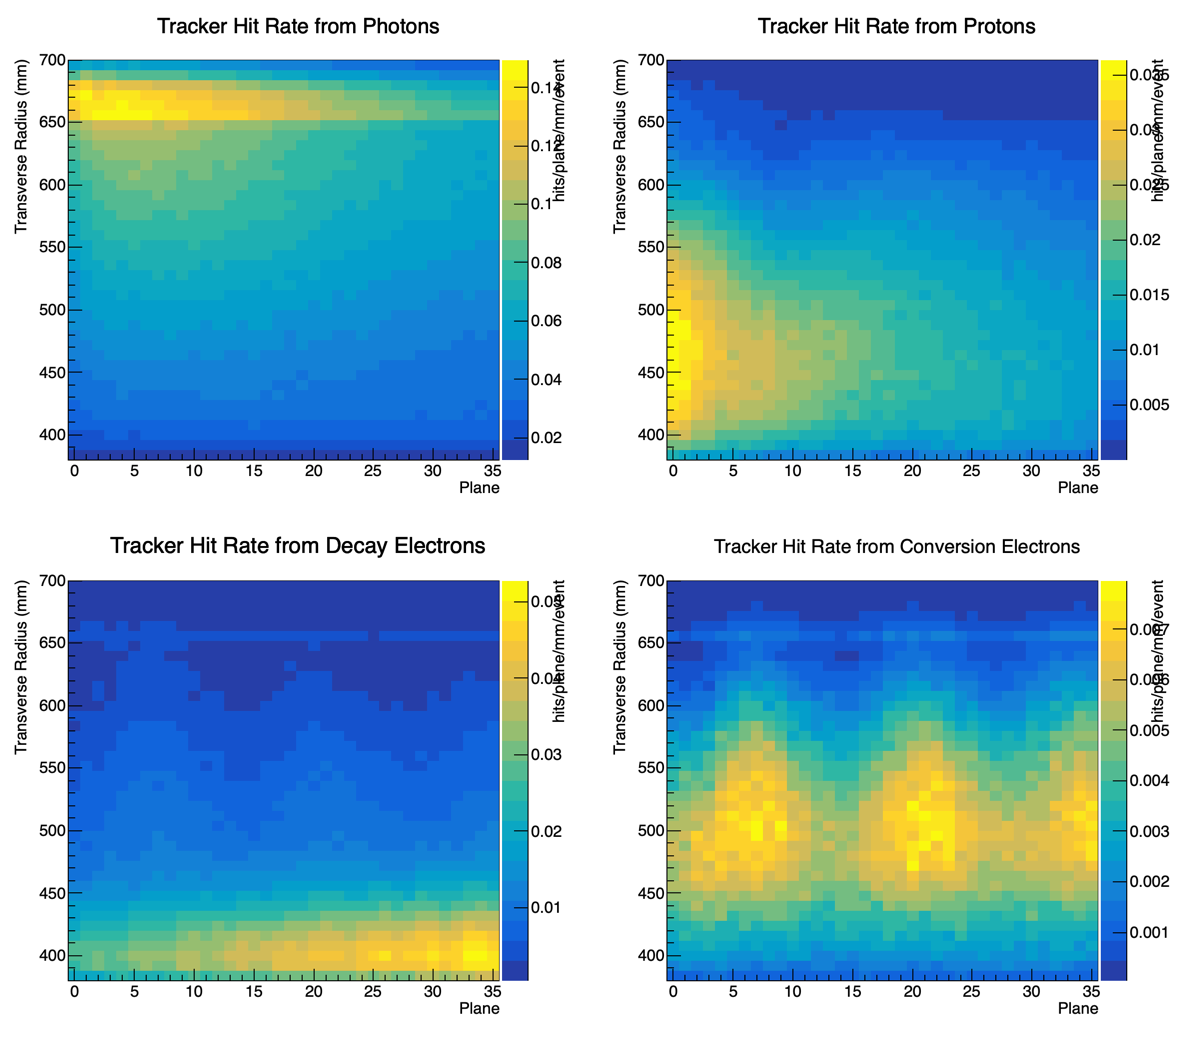
\includegraphics[width=\textwidth]{figures/trackerhits.png}%
 \caption{Track hit rate {\it vs} plane number and reconstructed transverse radius from different sources in simulated conversion electron events with beam pileup overlay.
 }%
 \label{fig:trackerhits}
\end{figure}

Hits from protons are removed using their large energy deposit. Hits from DIO are suppressed by requiring a minimum transverse radius, while hits originating from neutron capture in the DS are suppressed by requiring a maximum transverse radius. Hits from low-energy electrons are filtered using a dedicated algorithm that first clusters the hits in time and transverse position and then classifies the clusters using an ANN trained to separate low-energy from high-energy electrons by their geometric properties. The filtered hit collection passed to track pattern recognition has a signal purity of roughly 50\% in signal plus pileup simulation, inside the time window defined by the conversion electron hits.

\subsection{Signal Track Reconstruction}
The high-momentum track candidate search starts by looking for clusters of filtered hits with times within a sliding $\sim 50$ ns window. The hit time resolution is improved by roughly 30\% by subtracting the TOT-based drift time estimate. The hit straw Z position is used to correct the particle propagation time, dependent on the assumed or measured particle velocity.

Hits in a time cluster are passed to one of several helix finding algorithms, which extract rough helix parameters from the hit 3-D positions. Helix reconstruction is split into transverse (circle) and longitudinal phases, which are iterated between until convergence. One algorithm uses the position of high-energy (>50 \MeV) calorimeter clusters and the stopping target to seed the helix search, resulting in higher purity, but lower efficiency. The others use purely tracker information. Helices found by different algorithms that share the majority of their hits are merged. Helices from all algorithms use the same output data class. The performance of the different finding algorithms are similar, but not identical: in particular, the calorimeter-seeded algorithm is more robust against very high levels of pileup. As these algorithms are still being developed and tuned, and as they are easy to swap in and out and combine, Mu2e has not yet made a final decision on which ones will be used in the final trigger and reconstruction sequence.

Reconstructed helices are passed to a Kalman filter track fit to make final selections. The Mu2e fit uses the KinKal~\cite{Brown:2024tur} package, which is designed for precision kinematic reconstruction of low-momentum tracks in graded magnetic fields. The KinKal fit implements configurable simulated annealing, which allows for iterative pattern recognition and calibration refinement during the fit, and supports the integration of AI/ML pattern recognition tools as part of the fit. Within the KinKal framework, Mu2e has implemented a specialized track object, created fit constraint objects for both tracker hits and calorimeter clusters, and several ANN-based hit classification algorithms, which are applied as part of the annealing schedule. Associated calorimeter clusters are included as constraints on the fit time, allowing a more precise interpretation of the tracker hit drift time as a position constraint. The ANN classifiers remove residual background hits, refine the drift calibration, and help assign left-right ambiguities to tracker hits. 

Two configurations have been developed for the Mu2e KinKal fit, one optimized for use in the online trigger, and the other for offline analysis. The "trigger configuration" uses a minimal annealing schedule, a 1\% precision magnetic field correction, does not use track hit drift information, and does not add missing hits to the track. It provides a fit in roughly 5 msec/track processing time, with very high efficiency. The reconstructed momentum and the intrinsic momentum resolution using the trigger fit configuration for simulated conversion electron plus beam pileup events are shown in Fig.~\ref{fig:trigtrkmom}. Interpreting the full width half maximum (FWHM) of the momentum distribution as an effective core resolution using $\sigma = \rm FWHM/2.35$, the trigger fit achieves an absolute resolution of roughly $340 \keV$ down to the current trigger threshold of $80 \MeV$, which meets the Mu2e track trigger requirements~\cite{triggerreqs}.

\begin{figure}[tbp]
 \centering
 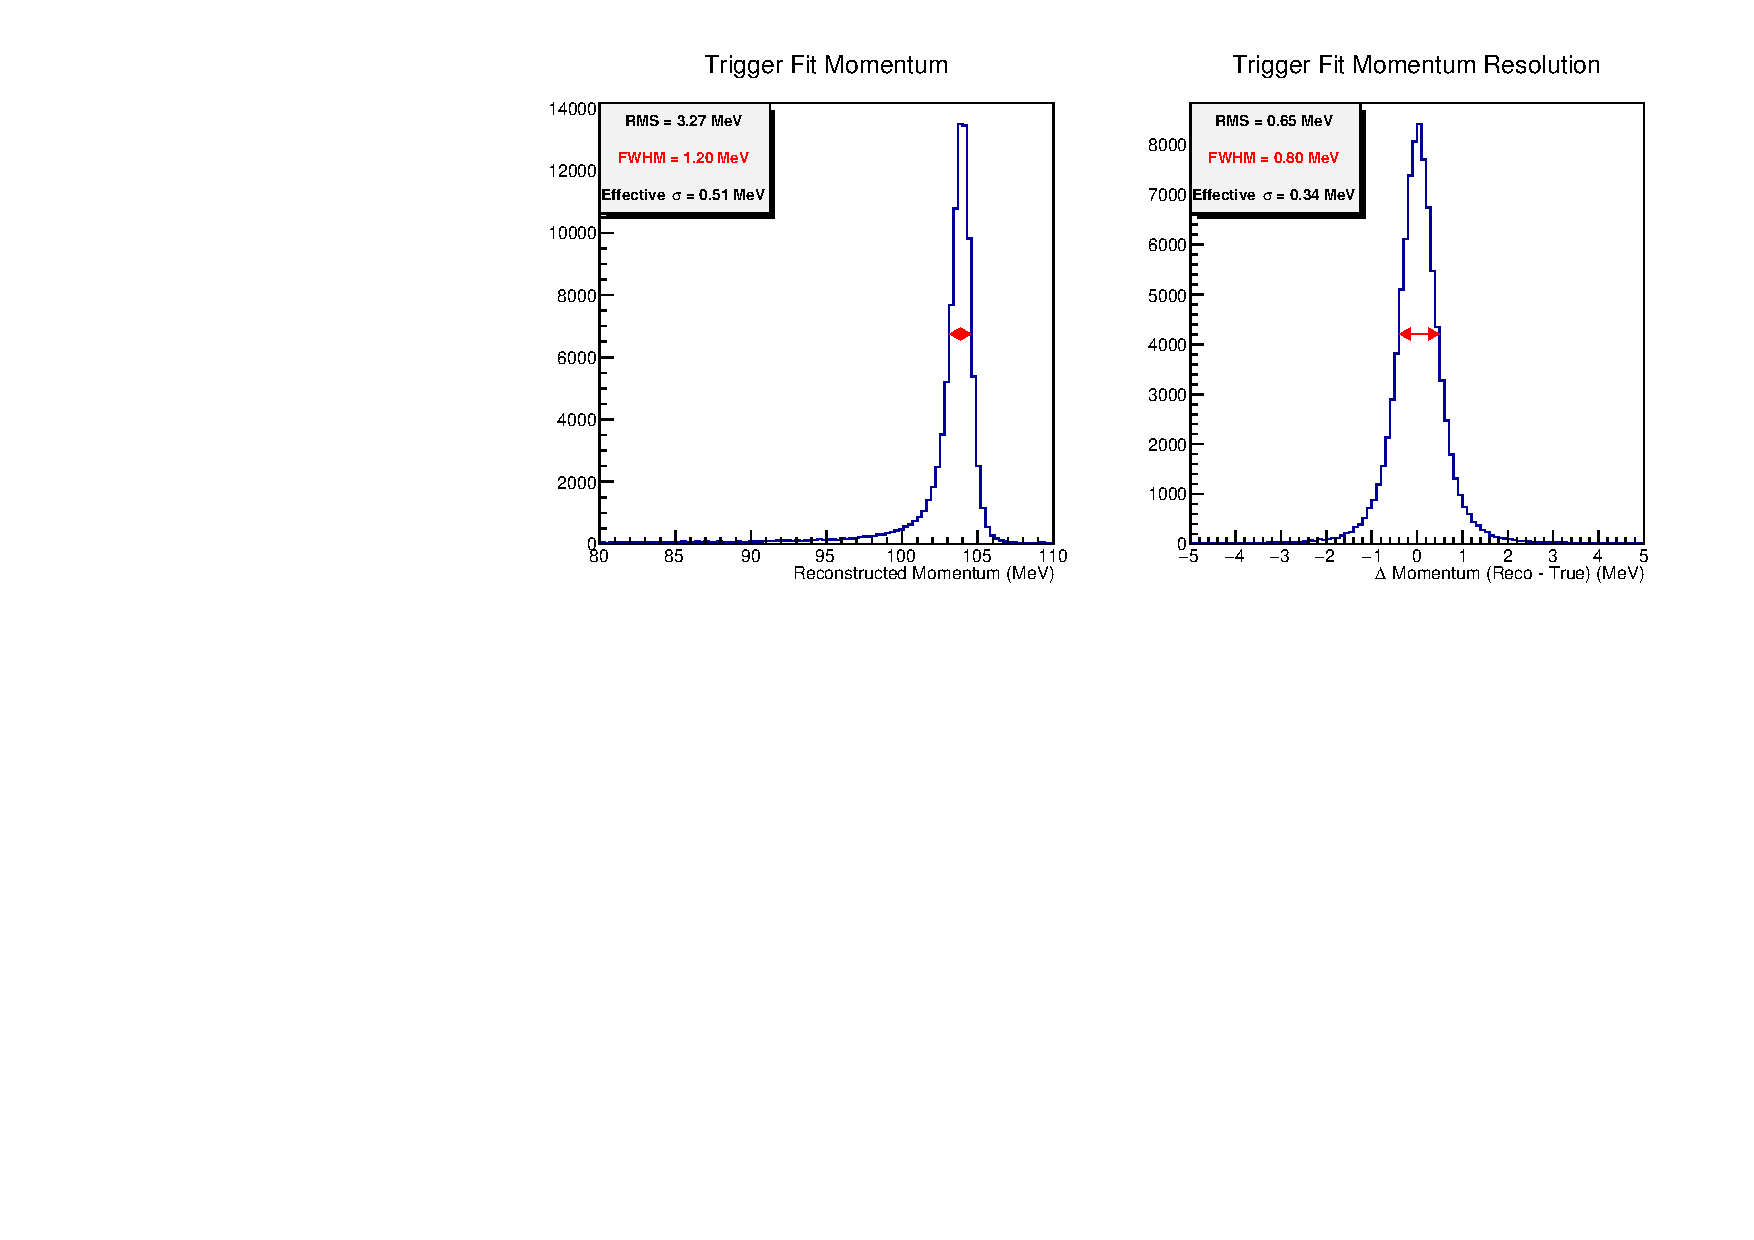
\includegraphics[width=\textwidth]{figures/KKTTmom.pdf}%
 \caption{Track momentum (left) and momentum resolution (right) in simulated conversion events with beam pileup overlay, reconstructed using the trigger KinKal configuration.}
 \label{fig:trigtrkmom}
\end{figure}

The "analysis configuration" uses a more gradual annealing schedule, a $10^{-4}$ precision magnetic field correction, full track hit drift information, and adds missing hits. This configuration requires roughly 50 msec/track, achieves essentially the same efficiency, and improved resolution. The reconstructed momentum and the intrinsic momentum resolution using the analysis fit configuration, sampled at the tracker entrance, for simulated conversion electron plus beam pileup events, are shown in Fig.~\ref{fig:anatrkmom}. 
%Interpreting the full width half maximum FWHM of the resolution distribution as an effective core resolution using $\sigma = FWHM/2.35$, we see 
The fit achieves an intrinsic resolution $\sigma = \rm FWHM/2.35 = 140 \keV$, exceeding the tracker requirement of $\sigma < 180 \keV$~\cite{trackerreqs}.

\begin{figure}[tbp]
 \centering
 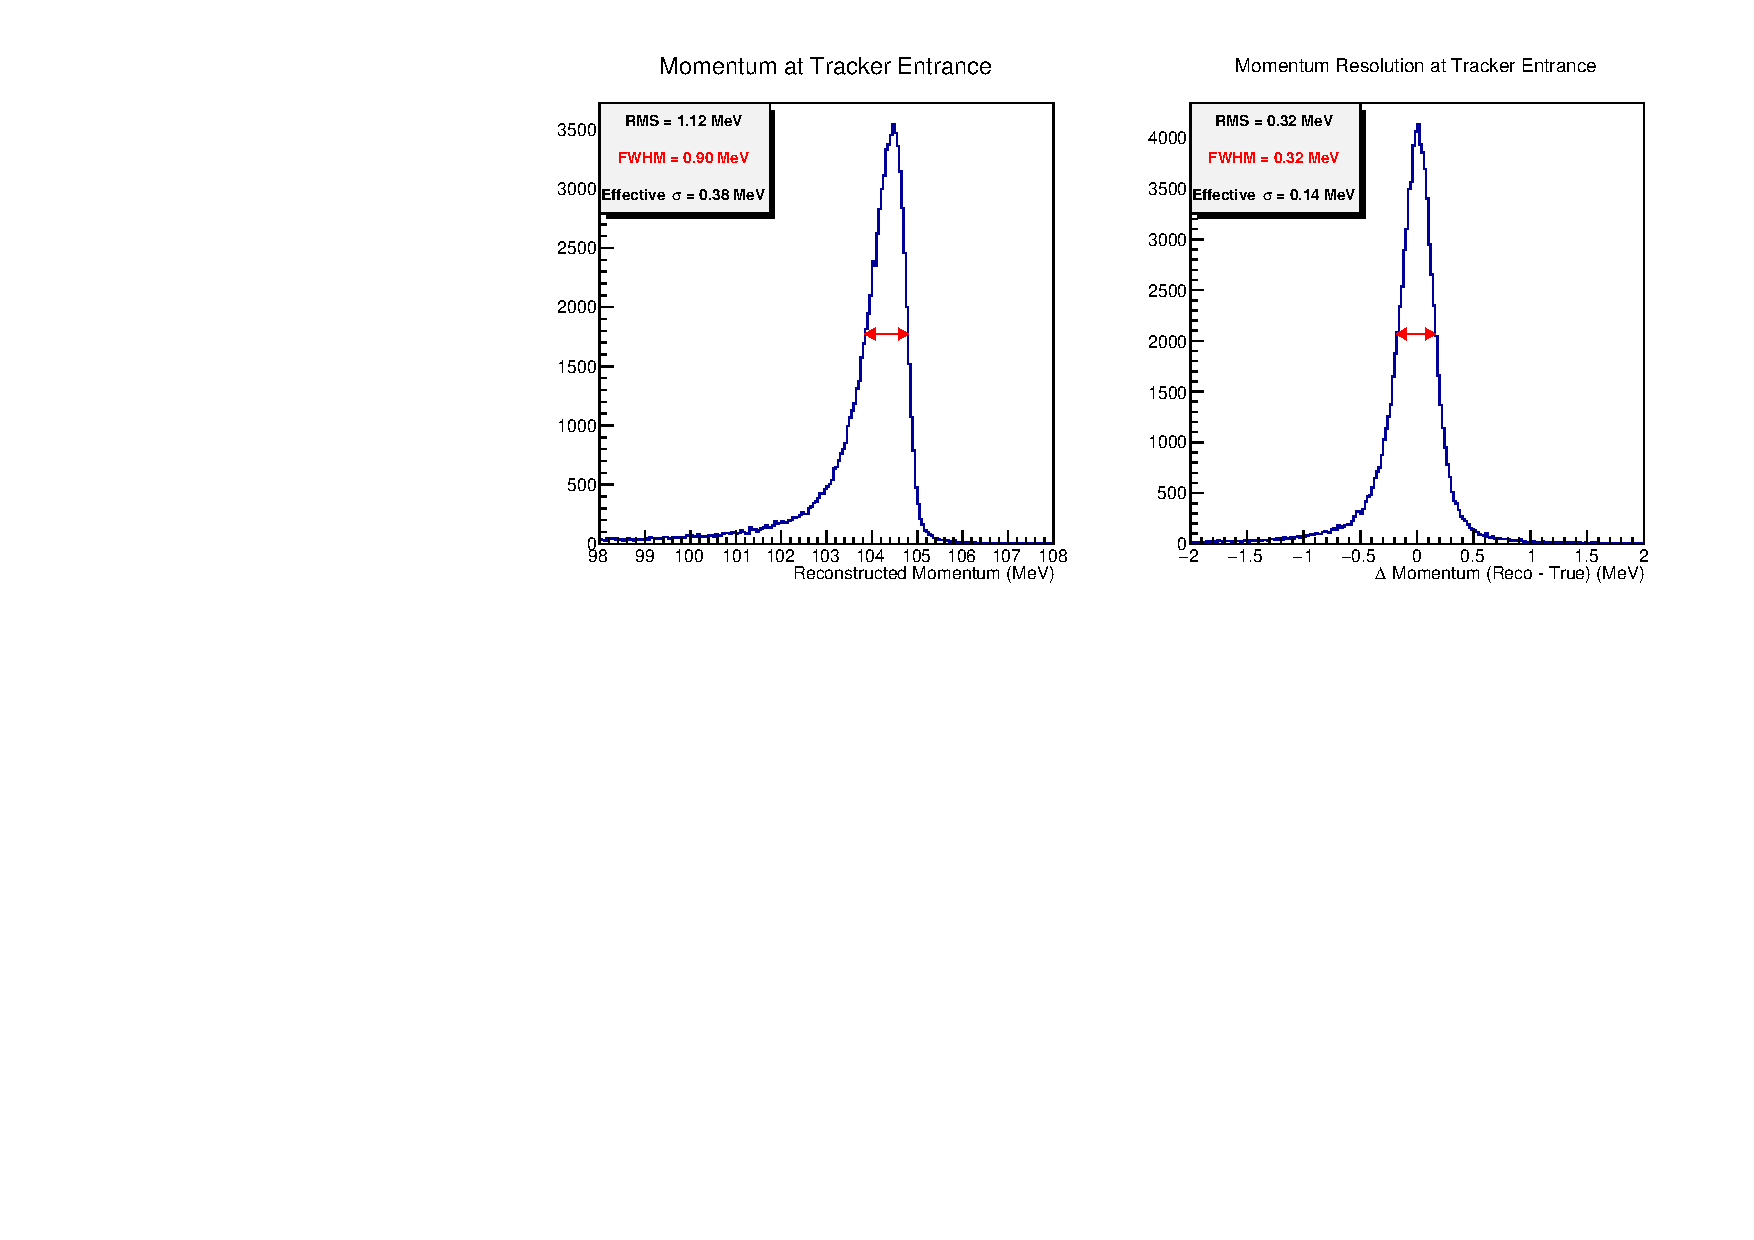
\includegraphics[width=\textwidth]{figures/KKMom.pdf}%
 \caption{Track momentum (left) and momentum resolution (right) sampled at the entrance to the tracker in simulated conversion events with beam pileup overlay, reconstructed using the analysis KinKal configuration (see text for definition).
 }%
 \label{fig:anatrkmom}
\end{figure}

As indicated by Fig.~\ref{fig:anatrkmom}, the absolute momentum resolution of Mu2e tracks is dominated by energy loss straggling in the stopping target and IPA. Evaluating the track momentum after extrapolation to the stopping target can potentially improve the absolute momentum resolution by accounting for estimated energy loss track-by-track instead of in aggregate. Algorithms to extrapolate reconstructed KinKal fit tracks beyond the fit region are under development. The core fit engine support for extrapolation is fully implemented and extrapolation in material-free regions has been demonstrated. The remaining task is the development of a KinKal model of the stopping target and IPA material and its integration with the fit.

\subsection{Straight Track Reconstruction}

The straight track reconstruction is used for cosmic ray tracks in the field-off configuration. As in the signal-track reconstruction, it begins by looking for clusters of filtered hits in time, but without attempting to correct for the particle propagation time. The straight line track seed also uses a simpler brute force algorithm. For each pair of straw hits, a straight line between the reconstructed hit positions is drawn and tested for intersections with the other hit straws, and the track with the highest number of successful intersections is chosen.

Two possible algorithms are used for the final reconstruction. First is a Kalman filter fit based on KinKal. Here the particle momentum is an input parameter that is held fixed during the fit. Similar to the signal fit, this fit can be configured to use a minimal annealing schedule and no drift information. In addition to making it faster, this configuration also makes it more robust against miscalibrations.

The second algorithm is a maximum likelihood fit that uses the ROOT Minuit2 minimizer. The likelihood for each straw hit includes both drift and longitudinal information, with the drift time likelihood for a given drift radius given by an exponentially modified Gaussian distribution that models the effect of both the random variations of the drift times for a single cluster and the exponential distribution of the effective drift distance given the discrete cluster statistics. The track is parameterized as a perfect straight line so no scattering is included. As a global fit, the results from this algorithm can easily be used with the Millepede-II alignment algorithm. 

\subsection{Calorimeter Reconstruction}

The data written by the calorimeter front-end electronics contains zero-suppressed waveforms recorded by the photo-sensors at the back of each crystal. These waveforms could be produced by a single or several particles depositing energy in a crystal during a short amount of time. In the latter case, the recorded waveform contains overlapping peaks, exhibiting multiple local maxima. The signal extraction procedure starts by fitting the waveform with an iterative procedure to extract the time and amplitude of each peak. The fit model is revised by adding or removing peaks until the chi-squared of the fit falls below a specified threshold (up to nine peaks can be extracted in a single waveform). The leading edge of the first peak is also refit to improve the timing resolution. The signal amplitudes are converted into energy deposits by using photosensor-specific calibration constants. The outputs of two photo-sensors within a time window of 4 ns are then merged to form crystal hits. 

Calorimeter clusters are finally formed by combining crystal hits. The most energetic hit is taken as a cluster seed, and all simply connected hits compatible with the seed time are added to the cluster content. These hits are then removed from the pool of available hits, and the procedure is repeated until all hits have been assigned to a cluster. A fraction of the particles interacting with the calorimeter produces one or more low-energy clusters near a more energetic one. A procedure is applied to combine these split-off clusters with the main cluster and improve the energy resolution. The energy, time, and other properties of the clusters are finally determined.

\subsection{CRV Reconstruction}
The CRV front-end boards record waveforms of each channel of the CRV detector. This is done in a non-zero-suppressed mode and a zero-suppressed mode, where the zero suppression threshold will be at around 5.5 photo-electrons. Non-zero-suppressed data is used for calibration purposes, and to validate the zero-suppression algorithm.

The zero-suppressed waveform data is used to reconstruct candidates of cosmic rays going through the CRV. First, individual waveforms are searched for pulses (local maxima), extracting the pulse time and pulse area. The pulse area is normalized by a channel-specific calibration constant (extracted from the conditions database) to obtain an estimate of the number of photo-electrons in this pulse.
%To distinguish CRV pulses that are caused by cosmic rays entering the detector (and may cause conversion-like electrons) from CRV pulses of other sources (e.g. beam-induced tracks), pulses in locally adjacent 
Based on the time, number of photo-electrons, and location of recorded CRV pulses, groups of pulses are associated with coincidence clusters. The current coincidence criterion requires pulses in 3 out of 4 CRV layers, with at least 10 photo-electrons, within 20 ns. Conversion electron candidates consistent in time and space with originating from a CRV coincidence cluster will be rejected (vetoed) in analysis. %Current algorithms achieve XXX rejection rate with a cost of YYY in signal candidate acceptance.
The CRV coincidence criteria and track consistency algorithms remain to be optimized for maximal acceptance while keeping the expected number of cosmic background tracks well below one.

\subsection{STM Reconstruction}
The STM data written by the DAQ consists of prescaled unsuppressed and zero-suppressed digitized waveforms as well the outputs of the online pulse processing algorithm, which consist of the uncalibrated energy and time of each hit. The unsuppressed and zero-suppressed waveforms are used to validate the online algorithms, and the outputs of the pulse-processing algorithms are used for the analysis. The pulse-processing algorithms have been tested at high rates using data collected in a test beam setup.

The outputs of the pulse-processing algorithms are calibrated in the Offline framework with calibration constants stored in the conditions service. We plot the energy spectrum of the calibrated hits and fit Gaussian functions to the peaks of interest in order to estimate the number of stopped muons. This method achieves a 10\% statistical uncertainty on the number of stopped muons with $\sim 10$ minutes of data in simulation. These $\sim$10-minute counts and associated uncertainties will be stored in a database. Event-by-event information such as the number of tracker hits or the total energy deposit in the calorimeter, can be used to interpolate between STM measurements to estimate the number of stopped muons per event.

\subsection{Extinction Monitor Reconstruction}

The reconstruction starts by grouping adjacent pixel hits from the same clock tick into clusters. The coordinates of a cluster are computed as the center of gravity of its component hits. The next step is pattern recognition. Straight line tracklets are formed from clusters in the upstream and, independently, downstream sensor stacks. A tracklet is constructed from 3 clusters; all in the same clock tick but in different planes. The position cuts are loose, allowing for a pixel-size misalignment error and a multiple scattering angle of up to 5 mrad in a plane. Upstream and downstream tracklets are matched into candidate tracks if they are in the same clock tick and if the angle difference in the non-bend projection for the tracklets is within $0.005$. A $\chi^2$ fit is performed on candidate tracks to determine 5 parameters: the starting position $(x,y)$ and direction at the detector entrance, and the bend radius in the magnet. 
%Figure~\ref{fig:extmonEff} Shows the extinction monitor track reconstruction efficiency as a function of particle multiplicity in simulation.
%\begin{figure}[tbp]
% \centering
% 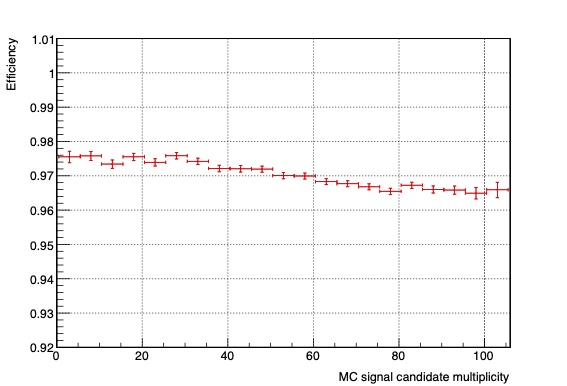
\includegraphics[width=\textwidth]{figures/extmonEff.png}%
% \caption{Track reconstruction efficiency vs particle multiplicity.
% }%
% \label{fig:extmonEff}
%\end{figure}


\section{Detector Calibration and Alignment}
\label{sec:calibration}

The calibration and alignment parameters needed by the reconstruction algorithms reside in the conditions database described below, along with the metadata allowing for versioning and defining the run/subrun range over which any set of calibration constants are valid. Several concurrent sets of calibrations will cover different use cases, for example, an initial set of values used during reconstruction for the trigger. Nominally, a given calibration set can be extended with values covering a new set of runs, allowing calibrated reconstruction to be performed on those runs. When calibration algorithms are updated or inputs are changed, a new version of the calibration set can be defined as well, possibly requiring reprocessing of relevant runs. The calibrations can also be overridden with text files, so iterating calibration procedures can easily include rerunning reconstruction using the previous step's results.

A large part of the calibration and alignment will be performed in situ, using cosmic ray or beam data collected during normal (including extracted position) Mu2e running conditions. There are also several sources of calibration data that will need dedicated setup and runs, including tracker charge injection pulsers, calorimeter laser system and DT source, Y-88 and Eu-152 sources for the stopping target monitor, etc. Most of these will also require specialized data processing. The various detector alignment procedures will also make use of metrology measurements made during both construction and after installation.

\subsection{Tracker calibration}

The majority of the tracker calibrations will be performed iteratively using data from reconstructed extracted or off-spill cosmic tracks. For extracted cosmics, the initial triggering and event selection is based on a simple time clustering of hits in the tracker. Each cluster is then reconstructed using both a KinKal Kalman filter track fit as well as a maximum likelihood-based straight-line track fit. Both track fit results are processed with Mu2e Offline modules to produce simplified output for calibration. 

Information from the KinKal fit is used to determine tracker calibration parameters from the TrkAna trees, including channel time offsets, time-to-distance relationships, and the TOT-to-drift time. Mean residuals for each channel are used to calculate corrections to the calibrations. Collecting a few thousand hits per channel requires around one day of extracted cosmic data.

The likelihood fit results are used to align the tracker modules with the Millepede-II algorithm~\cite{millepede1,millepede2}. Given a set of track fits Millepede-II performs a simultaneous least squares fit to all track parameters and alignment parameters, including correlations. It can be run interactively, taking only a few minutes to process millions of tracks. The Millepede fit can also include results from metrology measurements as Gaussian constraints on any linear combination of the alignment parameters. Separate 6-DOF alignment parameters are included for different levels of tracker modules, including each panel, plane, and the entire tracker. Redundant degrees of freedom are removed by applying fixed constraints within Millepede. We plan to eventually use KinKal fits of off-spill cosmic tracks for alignment as well, which should provide better constraints on systematic shifts and rotations. A track refit based on General Broken Lines~\cite{gbl} would allow us to reformulate the KinKal result and use Millepede again. 

Both the alignment and calibration are performed iteratively. Each iteration requires re-performing the hit and track reconstruction on the uncalibrated digi and producing a new set of data, but we expect the number of iterations to be small, even for initial bootstrapping. After convergence, the updated calibration and alignment parameters are uploaded to the condition database, and the calibration set can be extended to include new values to allow for pass-2 reconstruction. 

The ability to bootstrap the calibration and alignment using the first cosmic data was demonstrated using simulations. In the simulations, calibration and alignment parameters are set to randomly distributed values to model uncalibrated reconstruction. Additionally, parameters for the detector configuration like thresholds and channel statuses are varied. Simulations of cosmic data in the extracted position were produced using distributions of calibration parameters and states that model the expected condition of the detector for the initial data taking. The KinKal track fit with a reduced set of annealing steps is used for the first iteration of the calibration, after which the likelihood fit and full KinKal fit can be used for further steps. The performance of the calibrated track reconstruction is shown in Figure~\ref{fig:calibLong}. 


\begin{figure}[tbp]
  \centering
  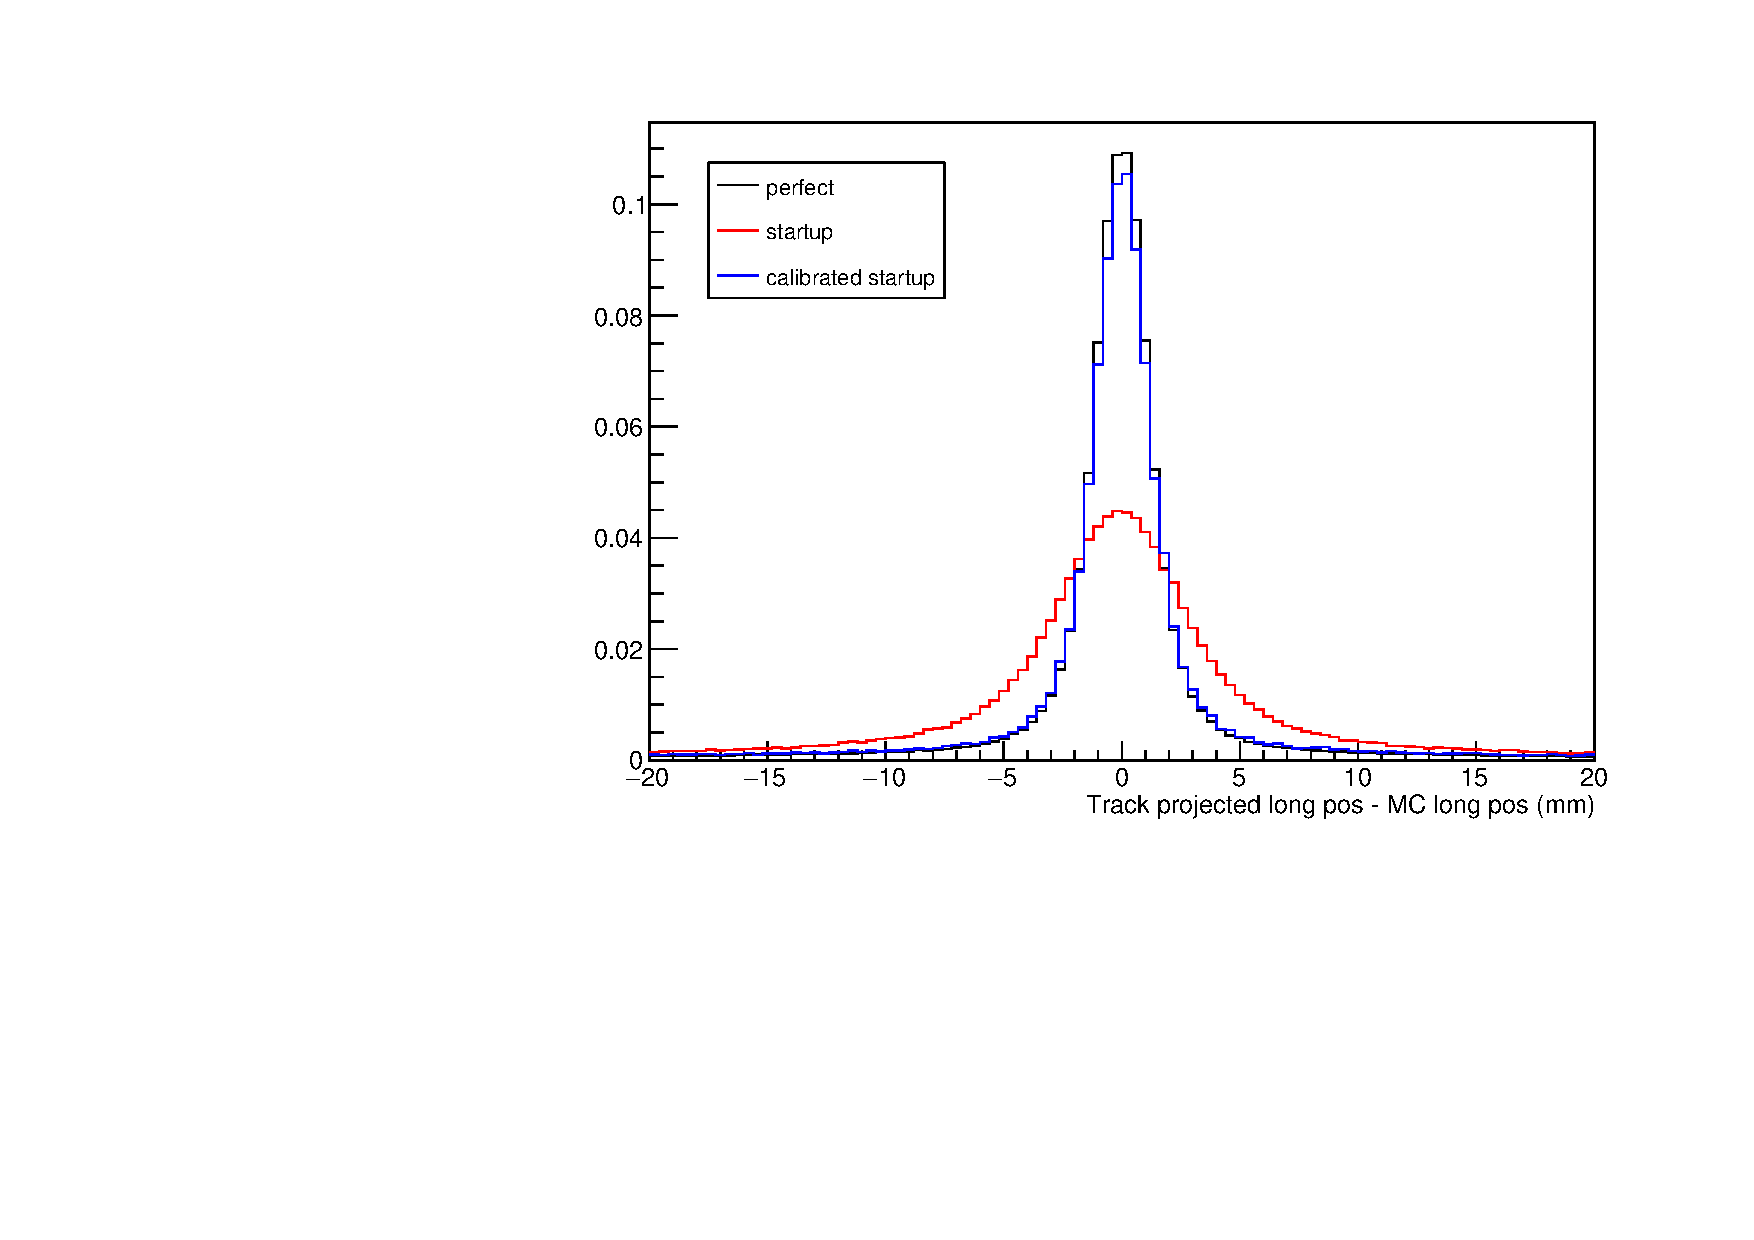
\includegraphics[height=0.4\textwidth]{figures/calibratedlong.pdf}%
  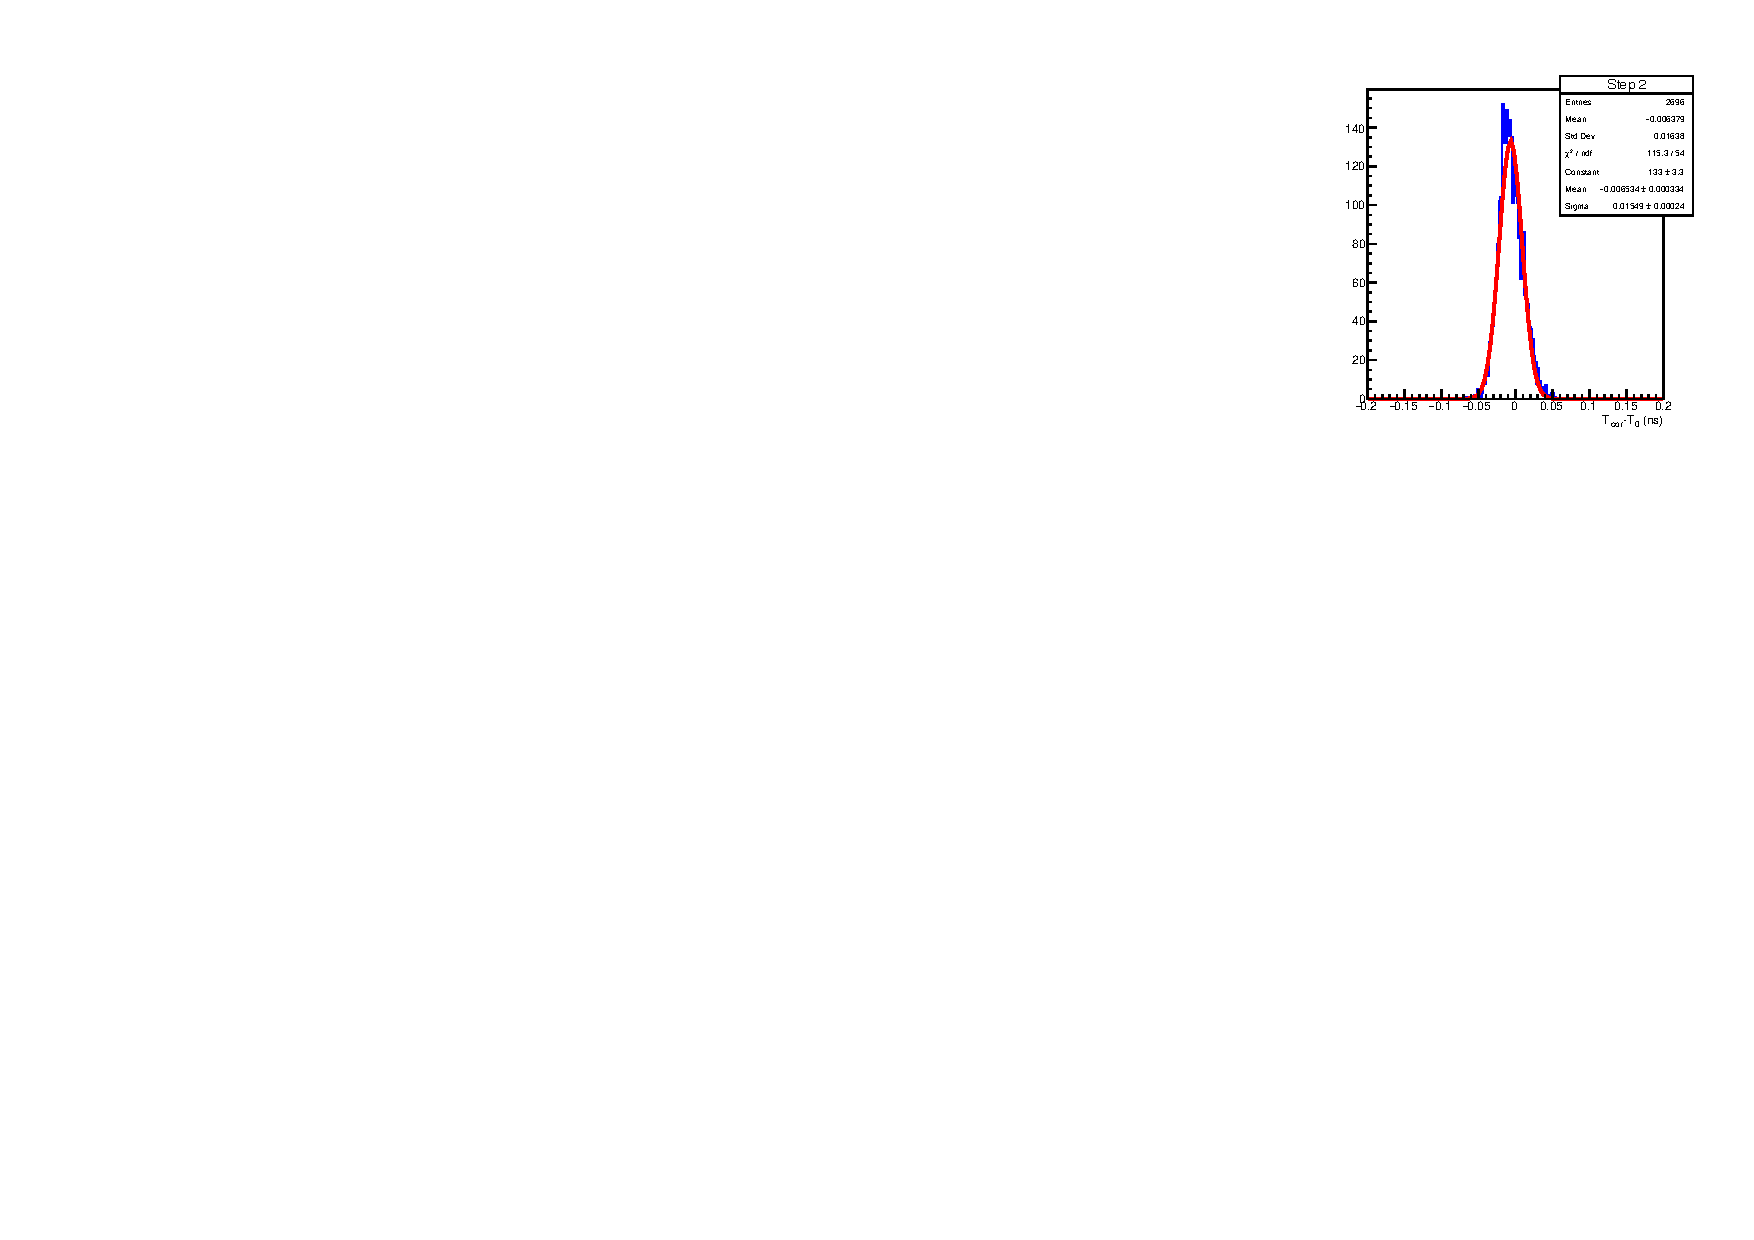
\includegraphics[height=0.4\textwidth]{figures/caloCalibTime.pdf}
  \caption{Left: Track fit longitudinal resolution in uncalibrated and calibrated simulated startup condition data as well as perfect simulated data. Right: Results of the calorimeter energy calibration procedure based on a simulated sample of cosmic rays equivalent to a data-taking period of 10 hours.}
  \label{fig:calibLong}
\end{figure}


\subsection{Calorimeter calibration}

The calorimeter makes use of three different calibration methods, based on the laser system, the source calibration systems, and cosmic ray events.

Cosmics calibration requires data samples in extracted position or off-spill during physics runs. The energy calibration is performed with minimum ionizing particles, identified as events with clusters from straight tracks with a minimum energy deposit. A $\sim 0.5\%$ spread is obtained from 10-hour simulated cosmic ray events in extracted position. The time calibration is performed in two steps. First, reconstructed hits produced by the laser are used to evaluate time offsets due to the electronics. The second step performs a least squares fit to clusters produced by minimum ionizing particles to calculate a correction to the time offsets for each channel. Simulation studies show that 15 ps time alignment is obtained. The energy and time calibration procedures have been validated using data collected by a large-scale calorimeter prototype containing 52 crystals. Results are consistent with MC expectations, demonstrating the robustness of the procedures.

The calorimeter has a radioactive source-based calibration system that allows for an absolute energy calibration of each crystal using a 6.13 MeV photon line. The distribution of reconstructed energy for each crystal is fit with 3 crystal ball functions, one for the main peak and two escape peaks, over a logistic background. This calibration has been tested using simulations that include crystal non-uniformity, electronics noise, and different photo-statistics, demonstrating consistency to less than one percent with data from a ten-minute long run. The laser system distributes green light to each calorimeter SiPM to perform a precise gain determination, with a dedicated run of a few minutes, and monitor the stability of the response by continuously firing a few pulses in the off-spill data collection period. Source and laser runs will be performed on a weekly basis.

The results from each calibration source are stored in "archive'' tables in the condition database (see Section~\ref{sec:databases}), and combined to produce the final calibration constants stored in the condition database. 

The calorimeter alignment is determined during construction using a laser tracker survey with a $\mathcal{O}(100\ \mu \text{m})$ accuracy on crystal position, enough for calorimeter reconstruction purposes. The geometrical alignment of the calorimeter will be completed once on the Mu2e detector train, through three aiming points placed on the calorimeter external structure. Cosmic ray events will then be used to determine the position and time alignment with respect to the tracker and the CRV.

\subsection{CRV calibration}

The CRV uses a special set of non-zero-suppressed waveforms for calibration, collected and digitized alongside normal data taking. The first stage processes the raw CRV digis and histograms the waveform values to calculate per channel pedestal values. Once pedestals have been calibrated, pulse reconstruction can be run, and an Offline module aggregates pulse heights and areas for dark rate pulses. A standalone script then fits for the single PE value for each channel.

This pulse calibration includes temperature corrections and requires data read out by the slow controls, both in the calibration process and in the calibrated pulse reconstruction. Initially, these temperatures are stored in a separate slow control database and are then imported into the reconstruction's conditions database at regular intervals (once every hour, depending on the temperature fluctuations in the Mu2e hall). Less than one second of non-zero-suppressed data is required for the full CRV pulse calibration.

Reconstruction and calibration of dark pulses from the non-zero-suppressed waveforms takes around 0.5 seconds per microbunch, or about 7 hours for the full pulse calibration dataset. These procedures have been demonstrated on data from several test stands so far.

%\begin{figure}[tbp]
%  \centering
%  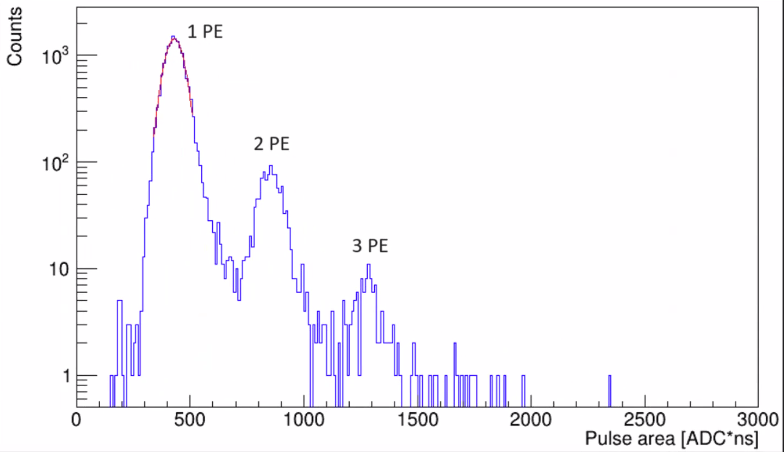
\includegraphics[width=0.5\textwidth]{figures/crvpulsefit.png}%
%  \caption{Output from CRV pulse reco from teststand data used to calibrate %pulse shapes. Single and multiple pe peaks are clearly seen.
%  }%
%  \label{fig:crvpulse}
%\end{figure}


\subsection{STM calibration}
The location of the STM and its collimation system is initially performed by optical survey. The relative alignment of the upstream and downstream structures will be then monitored by a laser alignment system to ensure that there are no large changes in the alignment that need to be corrected.

Acceptance and energy scale will be calibrated using Eu-152 and Y-88 sources. During data taking, the energy scale is expected to be stable over a few hours. Beam data will be used to monitor energy scale drift using various spectra lines (x-ray, gamma ray, 511 keV). Calibration constants will be stored in the conditions database. The time delay between the STM detectors and the other detectors can be measured using a scintillator paddle with a known cable length.

%\subsection{Extinction monitor calibration}
\section{Offline Data Quality Monitoring}
\label{sec:monitoring}
Describe how we plan to monitor Offlne data quality.  Describe the relationship with calibration.

\section{Physics Analysis}
\label{sec:analysis}

Data analysis broadly refers to the ensemble of tools and techniques used to extract constraints on the physical properties of the muon. Data analysis tasks include, for example, measurements of muon branching fractions and capture rates, comparisons between data and Monte Carlo simulations, extraction of calibration and detector performance parameters, or search for new phenomena. For these tasks, the software framework used for large-scale data processing might not be the most appropriate solution. This difference may not necessarily arise from missing functionalities or technological limitations in the large-scale production framework but might reflect the preference of analysts to trade capabilities in favor of flexibility and simplicity. The usage of external tools, such as machine learning or fit algorithms, might also be easier within a custom framework. Similarly, reduced data analysis samples (aka ntuples) might be more convenient to analyze than data containing the full event information. These samples could be structured differently from the data recorded by the detector (e.g. columnar structure) to improve the processing performance as well. This section describes the analysis frameworks and reduced data samples used by the experiment, together with a generic reference analysis based on these tools. While the development of a blinding strategy is of high importance for the collaboration, it is not expected to have a significant impact on computing and won't be discussed any further in this document. 




\subsection{Analysis Frameworks and Interfaces}

Offline analysis can be facilitated by using reduced data sets ("ntuples") consisting of a smaller set of physics variables deemed most useful for analyses. Information about low-level (hits) and high-level (tracks, clusters) products may need to be stored during commissioning and early data-taking periods. As the experiment matures, reduced ntupling scheme where only information from high-level data products is stored may become the default. Analysis groups will access these ntuples with either ROOT- or Python-based analysis scripts to create plots and perform statistical inferences to derive results.

To ensure operability on both FNAL and local resources, the ntuples data are stored as fundamental types instead of containing Mu2e-specific data products, removing the dependency on the full Mu2e software environment. Using the same assumptions and mock data samples as for the reconstruction output, the size of a ntuple dataset is estimated to be of the order of 100 GB (1 TB) if hit-level information is discarded (stored), small enough to be stored on persistent dCache (to avoid pre-staging the files from tape) or even locally. The simpler structure also translates into a shallower learning curve for new users since it can be easily accessed with ROOT and/or Python, the latter of which in particular is a common language used by early-career researchers.

Mu2e currently has two ntuple frameworks: TrkAna and Stntuple. Both output ROOT-based structures with data organized into event rows and containing reconstructed information extracted from Mu2e data products associated with the tracker, calorimeter, and CRV, as well as Monte Carlo truth information. TrkAna provides a simple ROOT TTree structure that can be accessed with ROOT or Python. Stntuple provides a separate lightweight interactive ntuple-based analysis framework based on that used by the CDF experiment at Fermilab. The Stntuple framework was ported to Mu2e and has evolved to meet the experiment's needs over several years. It supports multiple job configurations, interfaces with the data handling system, and has a built-in 2D event display. Stntuple was used for the \runone sensitivity estimate~\cite{Mu2e:2022ggl} and TrkAna is used for current mock data analysis efforts and to study cosmic ray alignment in the extracted position.

The framework is expected to evolve significantly in the near future with the definition of a single ntuple format satisfying most analysis needs and the development of interfaces with  modern analysis tools. This ntuple will necessarily have a "jagged" structure. For example, there will be different numbers and types (e.g. electron, muon) of reconstructed tracks in an event, and each track will include fit results from the Kalman fitter at different segments along the track (e.g. entrance of the tracker). The framework will provide simple interfaces to analyzers to manage this dimensional complexity and reduce the learning curve.

Analyzers will use either ROOT or Python to perform their analyses. ROOT-based analyses will use C/C++ macros, and Python-based analyses will use Python macros and/or Python notebooks. The ntuple is stored as a ROOT TTree so ROOT-based analyses will either loop through the TTree directly or use RDataFrames. RDataFrames have the advantage of performing "lazy" histogramming (i.e. define all cuts and histograms before looping through the data) and offering a transparent use of multi-threading capabilities. However, this would require code development to write RNtuples instead of TTrees, and we plan to evaluate the cost-benefit of this work during the long shutdown after \runone. Python-based analyses can access the data using ROOT via PyROOT or via the Python packages uproot and awkward array. Python-based analyzers can also use a wide range of available Python packages (e.g. numpy, scipy, hist) to perform their analyses. A common analysis environment is required to aid interoperability between groups and to ensure reproducible results. For ROOT-based analyses, a standard ROOT installation is maintained in Mu2e Offline, while a virtual environment will be provided for Python that can be easily recreated on local machines with either the venv or conda package managers. Tutorials and documentation of both Python- and ROOT C++-style analyses will be maintained throughout the experiment's lifetime. 

Machine learning (ML) algorithms are expected to play an important role in analysis-related tasks. Track quality and particle identification neural networks have already been trained in Python (with Tensorflow) and then evaluated in Mu2e Offline during the ntupling stage. For these, the ROOT TMVA::SOFIE interface is used to produce the C++ code to perform the calculation. New algorithms developed within the analysis groups will either be converted using TMVA::SOFIE and evaluated in the ntuple stage, or a common interface will be developed so that these tools are accessible to all analysis groups. ML algorithm training and other computing-intensive tasks (e.g. statistical inference with a large number of nuisance parameters) will leverage hardware accelerators and high-performance computing architectures to improve performance. The Elastic Analysis Facility (EAF) at FNAL could also be used to scale up data analysis: analysts can prototype their workflow on a subset of the data before seamlessly processing the full dataset. In any case, the computing needs for analysis are expected to be significantly lower than those needed for simulation and reconstruction.


\subsection{Reference Analysis}
% Some of the original material was moved to simulation or other section.
The Reference Analysis is developed to quantify the impact of software and algorithmic changes on the physics performance of the experiment; to prototype analysis tool; and to provide a cross-check to analysis groups. It takes input from the standard analysis framework in the form of reconstructed Mock Data developed using the output of large-scale ensemble production (see Section~\ref{subsec:ensembles}). In ensemnbles, conversion signals are combined with DIO tail backgrounds, cosmic backgrounds, radiative pion and muon capture backgrounds, and pile-up. The pile-up model contains contributions from neutral particles, beam electrons, and other muon processes such as decay in flight. The simulated data are then passed through the digitization and reconstruction framework to create samples similar to the data that will be collected by the DAQ system. 

Datasets equivalent to a year of data taking are created for two different $R_{\mu e}$, plus a no-signal scenario. A corresponding set of samples for the $\mu^{-}N \rightarrow e^{+}N'$ (including leading log corrections) is also produced. Digitization and reconstruction are simulated under two sets of calibration conditions: perfect and best. The "perfect" scenario describes a situation where the detector and digitization parameters behave in an ideal way, while the "best" scenario assumes more realistic conditions. As calibration algorithms evolve, more diverse sets of conditions could be simulated.

The current Reference Analysis contains signal extraction derived from two complementary and independent strategies: a simple counting experiment and an unbinned maximum likelihood fit. A few sources of systematic uncertainties will be added as nuisance parameters into the fit. Work to integrate the reference analysis into the validation workflow to track the evolution of reconstruction and analysis codes has begun.


\section{Databases}
\label{sec:databases}

The Mu2e database structure comprises several databases containing the metadata required to collect, store, process, and analyze data. An overview of information flow through Mu2e databases is shown in Figure~\ref{fig:db}. The subset of metadata needed to understand the data collected by the Mu2e detector is often referred to as condition data (e.g., detector alignment parameters or calibration constants). These data are indexed by (fraction of) runs, grouped into intervals of validity. Conditions data sampled at a lower frequency will be interpolated to match the physics requirements of the experiment. While conditions metadata will generally be stored in appropriate databases, they could be inserted in the raw detector data stream in some instances. APIs providing access to condition metadata independent of the underlying technical details will be provided to users. 

\begin{figure}[htb]
\begin{center}
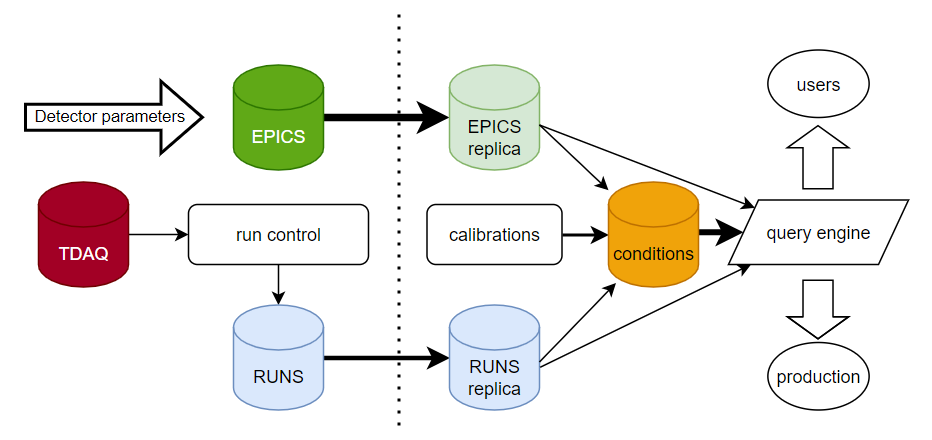
\includegraphics[width=0.8\linewidth]{figures/db.png}
\caption{An overview of information flow through Mu2e databases.}
\label{fig:db}
\end{center}
\end{figure}

Reliable access to metadata over the full lifetime of the experiment is a crucial requirement of the database system. To mitigate the risk that the underlying technology becomes obsolete during this period, Mu2e is following the general FNAL strategy of adopting open-source and widely supported products. The Mu2e DAQ system is based on MongoDB technology, while all other databases are using the PostgreSQL database management system. These databases are supported by the database group of the FNAL IT division, providing the software, the platform, and the servers (except the DAQ MongoDB database, hosted on the DAQ server to ensure continued access in case of network outage). All offline database accounts are authenticated by kerberos principles and are created by the database support group via a service desk ticket. The support group also provides a streaming service for copying from the online to the offline instance. The Mu2e workflow assumes 8/5 support for offline database with best effort outside standard hours.

All offline database content is written via SQL commands generated by Mu2e custom tools in c++ and python. Database queries are performed through the Query Engine, a lab-supported product providing an HTTP interface for all simple, high-rate queries. Two types of queries are available: reads from the web server cache (the cache refreshed with a programmable lifetime), or directly from the database via the web server. This system can be scaled to provide conditions content to jobs distributed across large numbers of grid-based or high-performance computing (HPC) systems. The service also provides valuable real-time monitoring of system response times and timelines. In addition, (partial) database content can be dumped into a file on /cvmfs and used for subsequent reconstruction or simulation tasks. This option could be useful in cases where the network bandwidth becomes limited, for example running a very large number of simulation jobs at a high-performance computing center.  

Database development is fully integrated into the Mu2e code development workflow and performed in collaboration with sub-system experts. A core principle is to maintain an automated robust audit trail of the processing history of each file, from TDAQ to final analysis datasets. This includes recording version information for code, databases and workflow configuration, and parent-child information among files. Mu2e has already recorded this information during the various simulation campaigns and we are investigating improved implementations. Among the desired features is the ability to specify that a file must be reprocessed using the same database versions that were used in the trigger.

The list of Mu2e databases is presented in Table \ref{tab:db}, and each instance is described in more detail below. 

\begin{table}[ht!]
\begin{center}
\begin{tabular}{ |l |c | c| }
\hline
label & schema & description \\ \hline
 DAQ & lab/Mu2e & DAQ configuration \\  
 EPICS & EPICS & detector metrics \\   
 run conditions & Mu2e & run metadata \\  
 offline EPICS & Mu2e & streamed from online \\  
 offline run conditions & Mu2e & streamed from online \\  
 conditions & Mu2e & calibrations \\
 DQM & Mu2e & offline data quality \\
 good run & Mu2e & good run list \\
 luminosity & Mu2e & runs luminosity \\
 SAM & lab & file metadata \\
 MetaCat & lab & file metadata \\
 Rucio & lab & file locations \\ \hline
\end{tabular}
\end{center}
\caption{Listing of Mu2e operations databases.  All are installed and managed by lab professionals.  All are postgres except DAQ, which is MongoDB.}
\label{tab:db}
\end{table}

%\begin{itemize}
%  \item DAQ configuration (online, not streamed offline)
%  \item run conditions database (online, streamed offline)
%  \item EPICS archive database (online, streamed offline)
%  \item conditions
%  \item good run
%  \item luminosity
%\end{itemize}


%\subsection{Infrastructure} \label{database-infrastructure}
%In implementing database infrastructure, we are following lab recommendations and leveraging lab expertise and support.  The DAQ database is MongoDB, but all other databases are version 14 pr 15 postgres.  The postgres databases are all hosted by the lab database group.  This support provides the postgress software, the platform, and servers. (Online database managed by the database group, but hosted on a Mu2e DAQ server.) All accounts are authenticated by kerberos principles and are created by the database support group via a servicedesk ticket.  The support group also provides a streaming service for copying from the online to offline instance.  Currently, the stream is up-to-date within 30 min, but this can be reduced to 10 min when needed.

%Offline, all database content is written by SQL commands generated by Mu2e tools, implemented using the psql exe at the command line, or libpq in c++ or psycopg2 in python.  All reads of the offline databases are through the Query Engine lab-supported product.  This system provides an http interface for all simple, high-rate database reads and is critical for providing conditions content to grid jobs.  Access is not authenticated, but is limited to on-site, VPN or select grid sites \red{need to re-check}.  There are two types of reads provided: reads from web server cache (the cache refreshed with a programmable lifetime), or directly from the database via the web server.  The service provides valuable real-time monitoring of system response times, including timelines.

%Mu2e has been operating with these systems for several years and we expect they will meet all our needs.


\subsection{Run Conditions database} 
The DAQ database is managed by the online operations group. At the beginning of each run, the DAQ system copies all information used to configure the detector and DAQ from the MongoDB DAQ database into the online run conditions database. Each run is divided into subruns, and the system records the precise times of the subruns in both wall clock time and accelerator ticks. At the end of the run, summary information (e.g. total number of processed events or run time) is added to the record. 

The online content is periodically streamed to an offline database instance. As a new run appears, offline data reconstruction is triggered and the job configuration is retrieved from the database. A web page with interactive search for data discovery also provides information about recent runs. Finally, tools are developed to extract the trigger configuration so that it can be reproduced for simulation or performance studies. 

\subsection{EPICS database}
EPICS is a system designed to monitor, display, and alarm arbitrary quantities, such as voltages, status, and environmental conditions. This stream of monitoring data is archived in an online postgres database using standard EPICS tools and then streamed to an offline instance. Users can access content through a simple custom tool (epicsTool), available both at the command line and in c++.

Environmental conditions required for detector response reconstruction is automatically extracted from the EPICS database offline instance and re-packaged in the conditions system to ensure reproducibility.

%Some detector responses are sensitive to environmental conditions. If this information is required in reconstruction, it is automatically extracted from the EPICS database offline instance and re-packaged in the conditions system for reproducibility.

\subsection{Conditions database} 
The conditions database tracks the detector conditions (e.g., pedestals, gains, bad channels,...) and their run dependence using a custom schema. The user specifies a purpose (such as "Pass~1'', "Sim2020'', or "CaloCalibration'') together with a version number to define which "conditions set'' the reconstruction job will access. The version number has three fields: the major version, used by experts to alert the user of an important change in conditions philosophy; the minor number,  indicating changes to content; and the final number, specifying the extension listing the intervals of validity. Reconstruction jobs with the same major and minor numbers will produce identical results, as a design requirement. The schema implements a closed interval of validity (with an option to relax if needed). When a repair is needed, or new types of tables need to be added, a new minor version is created.

Each detector sub-system defines the content of the tables added to the schema. In addition, "archive'' tables may be created to store intermediate results which are not used in reconstruction, but should still be saved. The system also provides "ad-hoc'' tables for secondary needs like record-keeping. A development database is available to verify the SQL commands and compatibility with code before creating the same table in the production environment. The content and intervals of validity provided by each sub-system are grouped into a condition set. 

A user interface dubbed "Proditions" provides access to the database in the reconstruction code. This layer can perform intermediate calculations based on the database contents and reorganize the data into different data structures or subsets of table data. The run-dependence of this content is automatically tracked based on the database table run dependence. Proditions has also an onboard cache to prevent thrashing.

Other implementation features include a text table option for overriding database content for testing purposes. Should the database access be unavailable, the text option can provide the entire conditions set content. A programmable onboard cache saves tables so switching back and forth between tables does not generate new fetches. All external operations are timed to evaluate the performance. Multiple layers of verbosity are provided to help debugging. The code is designed to be thread-safe as well.

All tools needed for database upload, queries, and repair have been developed. The conditions database system has already been extensively tested, and the measured performance will greatly exceed requirements for \passone, the most time-sensitive operation.  

%A development database exists with the identical schema as the production database. When a new calibration table is proposed, it is first installed in the development database to verify the SQL commands and compatibility with code, then the same table is created in production.  Other operations can be also tested first in development.  We have not found the need for an integration database yet, but if one is needed, it will be straightforward to create.

%Each subdetector defines what tables they need and they are added to the schema. The users may create "archive'' tables to store intermediate results which are not used in reconstruction, but should still be saved.  The system also provides "ad-hoc'' tables for secondary needs, like record-keeping. In operations, the subdetector expert provides content and IoV's, and passes them to the calibration coordinator, who joins the subdetector content together into a conditions set.

%All tools needed for database upload, readback, and repair exist.  The conditions database system has been in daily use for several years.  The system has been informally load-tested, and will greatly exceed requirements for pass1, the most time-sensitive operation.  A more formal load test will be coupled to raw data upload and pass1.


\subsection{DQM database} 
Data quality information may be produced at any stage of processing.  A set of analysis modules histogram critical quantities and the histogram files are preserved.  A series of tags label the files according to source, version, time, and run. A process then converts the histograms, and other information, into a series of metrics which are inserted in the DQM database. These metrics can be displayed as a function of run number or time or extracted as CSV tables for further analysis.  A system of limits provides alarms when metrics are out of tolerance.


\subsection{Good-run database} 
The definition of "good runs" will depend on the context and might involve input from the different detector sub-systems and experts. The good-run database collects information relative to run quality (typically an int) for a given interval of validity. Users can retrieve and edit this information to create a custom selection, which is then persistent in the database. The data can be accessed either by dedicated tools or within the reconstruction software. 

%Different analysis groups may define what is usable data differently and should have the ability to define what runs they want to use for a given purpose.  What is considered good may also involve input from many sub-system and other experts. The good-run database collects input from experts, as a status (typically an int) for a given IoV.  The user of these, then can define a selection, of these reports, add information from run conditions, adjust the selection by hand, then preserve the selection in the database.  Access to the good run list is by tools, or as a filter in processing.

\subsection{Luminosity database}
The number of stopped muons must be known to properly normalize the experimental results. To this end, it may be useful to track the number of protons on the primary target and other experimental quantities (e.g. the number of protons in the tracker), possibly as frequently as every micro-bunch. This large amount of data would be preserved in a database and accessed using custom tools or within the reconstruction software.

\subsection{Data-handling databases}
The data-handling database is fully designed and managed by the lab and contains standard schema. All writes are by standard tools with standard authentication systems. All reads are via load-balanced http services designed and maintained by the lab. The SAM database is a legacy system and will be deprecated before full operations.

%The number of stopped muons is the denominator in the measurement or limit for charge lepton flavor violation, the primary goal of Mu2e.  Towards this end, it may be useful to track the number of protons on the primary target, possibly as frequently as every bunch.  We will track several quantities per proton bunch, resulting in a large dataset.  We expect this will be preserved in a database, and accessed using custom tools, as an efficiency-weighted luminosity independent, of event processing on the grid. (XXX this section is weak)

\section{Software Management (Rob)}
\label{sec:codemanagement}
Mu2e uses github to manage our code.  We have multiple repos (list Offline repos).  We use CI testing and commit hooks and clangtidy to monitor quality. Describe code build tools and distribution to users and grid jobs.

\section{Communication Tools}
Tools used for Offline computing communication include slack, doc-db, email lists.


\section{Estimated Computing Resource Needs}
\label{sec:resources}
Give a history of previous resource estimates and the timeline.
Give the current underpinning numbers for the resource estimates.
Describe the manpower resource estimates, both CSAID and collaboration.
Describe computing resources available across the collaboration (FNAL, INFN, NERSC, EAF, ...) and our plan for using those.


Where should we describe the harvesting of online data?

\appendix
\section{Timeline of Offline Computing Milestones}
\label{sec:timeline}
timeline of developments

\section{Computing Model Definition (temporary reference only)}
A Computing Model is a bottoms up calculation of the time profile of computing resources needed by the experiment, starting now and extending until the final publication. The granularity of the time profile should be fine enough to identify peak usage needs. The level of detail should be appropriate for the maturity of the experiment and nearness to data taking.
It should include our needs for:
\begin{enumerate}
  \item CPU
    \begin{enumerate}
      \item Broken down by type of usage (see below for the definition of “type of usage”).
      \item Broken down by Fermigrid, OSG, HPC center and collaboration contributed CPU.
      \item For Fermigrid and OSG usage, this should be expressed in terms of memory
      \item Identify when there will be needs for jobs with unusually high memory needs.
    \end{enumerate}

  \item GPU and other non-CPU computing
  \item Disk and tape needs
    \begin{enumerate}
      \item Broken down by type of usage
      \item A bottoms up usage model that predicts the size of persistent dCache needed for
        each workflow in order to minimize tape activity for transient files.
    \end{enumerate}
  \item Network
    \begin{enumerate}
      \item Broken down by type of usage Network bandwidth:
      \item On-site
      \item Wide area, to support use of off-site CPU resources, including resources out of
        the country and collaborator contributed resources.
    \end{enumerate}

  \item  Databases
    \begin{enumerate}
      \item types of database.  For each type give:
      \item What is its expected final size?
      \item How often will it be updated?
      \item Does it need to be served via QueryEngine?
    \end{enumerate}
\end{enumerate}
 % this is temporary for reference only

%
% BibTeX or Biber users please use (the style is already called in the class, ensure that the "woc.bst" style is in your local directory)
% \bibliography{name or your bibliography database}
%
% Non-BibTeX users please use
%
\begin{thebibliography}{}
%
% and use \bibitem to create references.
%
%\bibitem{RefJ}
% Format for Journal Reference
%Journal Author, Journal \textbf{Volume}, page numbers (year)
% Format for books
%\bibitem{RefB}
%Book Author, \textit{Book title} (Publisher, place, year) page numbers
\bibitem{Mu2e} Mu2e Technical Design report
\end{thebibliography}

\end{document}

% end of file template.tex

<div id='footer'><table width='100%'><tr><td class='right'><a href='http://fusioninventory.org/'><span class='copyright'>FusionInventory 9.1+1.0 | copyleft <img src='/glpi/plugins/fusioninventory/pics/copyleft.png'/>  2010-2016 by FusionInventory Team</span></a></td></tr></table></div>
